
\providecommand{\pandocbounded}[1]{#1}
\makeatletter
\def\maxwidth{\ifdim\Gin@nat@width>\linewidth\linewidth\else\Gin@nat@width\fi}
\def\maxheight{\ifdim\Gin@nat@height>\textheight\textheight\else\Gin@nat@height\fi}
\makeatother
\providecommand{\tightlist}{\setlength{\itemsep}{0pt}\setlength{\parskip}{0pt}}
\chapter{Dữ liệu nguyên thủy và vòng lặp xác định}
\section{Chương 2: Dữ liệu Nguyên thủy và Vòng lặp Xác định (Primitive
Data and Definite
Loops)}\label{chux1b0ux1a1ng-2-dux1eef-liux1ec7u-nguyuxean-thux1ee7y-vuxe0-vuxf2ng-lux1eb7p-xuxe1c-ux111ux1ecbnh-primitive-data-and-definite-loops}

\subsection{Giới thiệu}\label{giux1edbi-thiux1ec7u}

Bây giờ bạn đã biết đôi chút về cấu trúc cơ bản của một chương trình
Java, bạn đã sẵn sàng để học cách giải quyết các bài toán phức tạp hơn.
Trong thời gian tới, chúng ta sẽ vẫn tập trung vào các chương trình tạo
ra đầu ra (output), nhưng chúng ta sẽ bắt đầu khám phá một số khía cạnh
của lập trình đòi hỏi kỹ năng giải quyết vấn đề.

Nửa đầu của chương này lấp đầy hai mảng quan trọng. Thứ nhất, nó xem xét
các biểu thức (expressions), được sử dụng để thực hiện các tính toán đơn
giản trong Java, đặc biệt là các tính toán liên quan đến dữ liệu số. Thứ
hai, nó thảo luận về các phần tử chương trình được gọi là các biến
(variables) có thể thay đổi giá trị trong khi chương trình thực thi.

Nửa sau của chương giới thiệu cấu trúc điều khiển đầu tiên của bạn: vòng
lặp \texttt{for} (for loop). Bạn sử dụng cấu trúc này để lặp lại các
hành động trong một chương trình. Điều này hữu ích bất cứ khi nào bạn
tìm thấy một khuôn mẫu (pattern) trong một tác vụ, chẳng hạn như việc
tạo ra một hình phức tạp, bởi vì bạn có thể sử dụng một vòng lặp
\texttt{for} để lặp lại hành động nhằm tạo ra khuôn mẫu cụ thể đó. Thử
thách là tìm ra mỗi khuôn mẫu và chỉ ra những hành động lặp lại nào sẽ
tái tạo lại nó.

Vòng lặp \texttt{for} là một cấu trúc điều khiển linh hoạt có thể được
sử dụng cho nhiều tác vụ. Trong chương này, chúng ta sử dụng nó cho các
vòng lặp xác định (definite loops), nơi bạn biết chính xác bạn muốn thực
hiện một tác vụ cụ thể bao nhiêu lần. Trong Chương 5, chúng ta sẽ thảo
luận về cách viết các vòng lặp không xác định (indefinite loops), nơi
bạn không biết trước mình sẽ thực hiện một tác vụ bao nhiêu lần.

\begin{center}\rule{0.5\linewidth}{0.5pt}\end{center}

\subsection{Các khái niệm Dữ liệu Cơ bản (Basic Data
Concepts)}\label{cuxe1c-khuxe1i-niux1ec7m-dux1eef-liux1ec7u-cux1a1-bux1ea3n-basic-data-concepts}

Các chương trình thao tác với thông tin, và thông tin có nhiều dạng.
Java là một ngôn ngữ an toàn kiểu (type-safe language), có nghĩa là nó
yêu cầu bạn phải nêu rõ loại thông tin nào bạn dự định thao tác và nó
đảm bảo rằng bạn thao tác dữ liệu một cách hợp lý. Mọi thứ bạn thao tác
trong một chương trình Java sẽ thuộc một kiểu nhất định và bạn sẽ liên
tục phải báo cho Java biết những kiểu dữ liệu nào bạn dự định sử dụng.

\begin{quote}
\textbf{Kiểu dữ liệu (Data Type)} Tên gọi cho một danh mục các giá trị
dữ liệu có liên quan với nhau, chẳng hạn như kiểu \texttt{int} trong
Java, được sử dụng để biểu diễn các giá trị số nguyên.
\end{quote}

Một quyết định đã được đưa ra ngay từ đầu trong thiết kế của Java là hỗ
trợ hai loại dữ liệu khác nhau: dữ liệu nguyên thủy (primitive data) và
đối tượng (objects). Các nhà thiết kế đã đưa ra quyết định này hoàn toàn
vì lý do hiệu năng, để làm cho các chương trình Java chạy nhanh hơn.
Thật không may, điều đó có nghĩa là bạn phải học hai bộ quy tắc về cách
dữ liệu hoạt động, nhưng đây là một trong những lúc bạn đơn giản là phải
trả giá nếu muốn sử dụng một ngôn ngữ lập trình ở đẳng cấp công nghiệp.
Để làm cho mọi thứ dễ dàng hơn một chút, chúng ta sẽ nghiên cứu các kiểu
dữ liệu nguyên thủy trước tiên, trong chương này; ở chương tiếp theo,
chúng ta sẽ chuyển hướng chú ý sang các đối tượng.

\subsubsection{Các Kiểu Nguyên thủy (Primitive
Types)}\label{cuxe1c-kiux1ec3u-nguyuxean-thux1ee7y-primitive-types}

Có tám kiểu dữ liệu nguyên thủy trong Java: \texttt{boolean},
\texttt{byte}, \texttt{char}, \texttt{double}, \texttt{float},
\texttt{int}, \texttt{long}, và \texttt{short}. Bốn trong số này được
coi là cơ bản: \texttt{boolean}, \texttt{char}, \texttt{double}, và
\texttt{int}. Bốn kiểu còn lại là các biến thể tồn tại cho các chương
trình có yêu cầu đặc biệt.

Bốn kiểu cơ bản mà chúng ta sẽ khám phá được liệt kê trong Bảng 2.1.

\textbf{Bảng 2.1 Các kiểu nguyên thủy thường dùng trong Java} \textbar{}
Kiểu (Type) \textbar{} Mô tả \textbar{} Ví dụ \textbar{}
\textbar---\textbar---\textbar---\textbar{} \textbar{} \texttt{int}
\textbar{} Số nguyên (integer) \textbar{} 42, -3, 0 \textbar{}
\textbar{} \texttt{double} \textbar{} Số thực (real number) \textbar{}
3.14, -0.5 \textbar{} \textbar{} \texttt{char} \textbar{} Ký tự
(character) \textbar{} `a', `X', `!' \textbar{} \textbar{}
\texttt{boolean} \textbar{} Giá trị logic (boolean) \textbar{} true,
false \textbar{}

Các tên kiểu (\texttt{int}, \texttt{double}, \texttt{char}, và
\texttt{boolean}) là các từ khóa (keywords) của Java mà bạn sẽ sử dụng
trong chương trình của mình để cho Trình biên dịch (Compiler) biết rằng
bạn có ý định sử dụng kiểu dữ liệu đó.

Có vẻ kỳ quặc khi sử dụng một kiểu cho số nguyên và một kiểu khác cho số
thực. Chẳng phải mọi số nguyên đều là số thực sao? Câu trả lời là có,
nhưng đây là các loại số hoàn toàn khác nhau. Sự khác biệt lớn đến mức
chúng ta thực hiện sự phân biệt này ngay cả trong tiếng Anh (và tiếng
Việt).

Trong lập trình, sự phân biệt này còn quan trọng hơn, bởi vì số nguyên
và số thực được biểu diễn theo những cách khác nhau trong bộ nhớ của máy
tính: Số nguyên được lưu trữ chính xác (exactly), trong khi số thực được
lưu trữ dưới dạng các giá trị xấp xỉ (approximations) với một số lượng
chữ số có nghĩa giới hạn. Bạn sẽ thấy rằng việc lưu trữ giá trị dưới
dạng xấp xỉ có thể dẫn đến các sai số làm tròn (round-off errors) khi
bạn sử dụng giá trị thực.

\subsection{Biến (Variables)}\label{biux1ebfn-variables}

Dữ liệu nguyên thủy có thể được lưu trữ trong bộ nhớ của máy tính dưới
dạng một biến (variable).

\begin{quote}
\textbf{Biến (Variable)} Một vị trí bộ nhớ có tên và kiểu dùng để lưu
trữ một giá trị.
\end{quote}

Hãy hình dung bộ nhớ của máy tính giống như một bảng tính khổng lồ
(spreadsheet) có nhiều ô nơi dữ liệu có thể được lưu trữ. Khi bạn tạo
một biến trong Java, bạn đang yêu cầu nó dành riêng một trong những ô đó
cho biến mới này. Ban đầu ô sẽ trống, nhưng bạn sẽ có tùy chọn lưu trữ
một giá trị vào ô đó. Và giống như với một bảng tính, bạn sẽ có tùy chọn
thay đổi giá trị trong ô đó sau này.

Tuy nhiên, Java kén chọn hơn một chút so với một bảng tính, ở chỗ nó yêu
cầu bạn phải cho nó biết chính xác loại dữ liệu nào bạn sẽ lưu trữ trong
ô. Ví dụ, nếu bạn muốn lưu trữ một số nguyên, bạn cần cho Java biết rằng
bạn dự định sử dụng kiểu \texttt{int}. Nếu bạn muốn lưu trữ một số thực,
bạn cần cho Java biết rằng bạn dự định sử dụng \texttt{double}. Bạn cũng
phải quyết định một cái tên để sử dụng khi bạn muốn tham chiếu đến vị
trí bộ nhớ này. Các quy tắc thông thường của định danh (identifiers)
trong Java được áp dụng (tên phải bắt đầu bằng một chữ cái, có thể được
theo sau bởi bất kỳ kết hợp nào của chữ cái và chữ số). Quy ước tiêu
chuẩn trong Java là bắt đầu tên biến bằng một chữ cái viết thường, chẳng
hạn như \texttt{number} hoặc \texttt{digits}, và viết hoa bất kỳ từ nào
theo sau, chẳng hạn như \texttt{numberOfDigits}.

Để khám phá việc sử dụng cơ bản của các biến, hãy xem xét một chương
trình tính toán chỉ số khối cơ thể (BMI - body mass index) của một cá
nhân. Các chuyên gia y tế sử dụng con số này để khuyên mọi người về việc
họ có bị thừa cân hay không. Cho trước chiều cao và cân nặng của một cá
nhân, chúngua có thể tính toán BMI của người đó. Khi đó, một chương
trình BMI đơn giản, một cách tự nhiên sẽ có ba biến cho ba mảnh thông
tin này.

Có một vài chi tiết mà chúng ta cần thảo luận về các biến, nhưng việc
nhìn vào một chương trình hoàn chỉnh trước để thấy bức tranh tổng thể có
thể sẽ hữu ích. Chương trình sau tính toán và in ra BMI cho một cá nhân
cao 5 feet 10 inches và nặng 195 pounds:

\begin{verbatim}
 1  // Computes Body Mass Index (BMI) for a specific person.
 2  public class BMICalculator {
 3      public static void main(String[] args) {
 4          // declare variables
 5          double height;
 6          double weight;
 7          double bmi;
 8
 9          // compute BMI
10          height = 70;
11          weight = 195;
12          bmi = weight / (height * height) * 703;
13
14          // print results
15          System.out.println("Current BMI:");
16          System.out.println(bmi);
17      }
18  }
\end{verbatim}

Lưu ý rằng chương trình bao gồm các dòng trống để tách biệt các phần và
các chú thích (comments) để chỉ ra các phần khác nhau của chương trình
làm gì. Nó tạo ra đầu ra (output) như sau:

\begin{verbatim}
Current BMI: 
27.976530612244897
\end{verbatim}

Bây giờ hãy kiểm tra các chi tiết của chương trình này để hiểu cách các
biến hoạt động. Trước khi các biến có thể được sử dụng trong một chương
trình Java, chúng phải được khai báo (declared). Dòng mã khai báo biến
được gọi là khai báo biến (variable declaration).

\begin{quote}
\textbf{Khai báo (Declaration)} Một yêu cầu dành riêng một biến mới với
một tên và một kiểu cho trước.
\end{quote}

Mỗi biến chỉ được khai báo một lần duy nhất. Nếu bạn khai báo một biến
nhiều hơn một lần, bạn sẽ nhận được một thông báo lỗi từ trình biên dịch
Java. Khai báo biến đơn giản có dạng:

\begin{verbatim}
<type> <name>;
\end{verbatim}

chẳng hạn như ba khai báo ở đầu chương trình mẫu của chúng ta:

\begin{verbatim}
double height;
double weight;
double bmi;
\end{verbatim}

Lưu ý rằng một khai báo biến, giống như một câu lệnh (statement), kết
thúc bằng một dấu chấm phẩy (;). Các khai báo này có thể xuất hiện ở bất
cứ nơi nào một câu lệnh có thể xảy ra. Khai báo chỉ định kiểu và tên của
biến. Hãy nhớ rằng tên của mỗi kiểu nguyên thủy là một từ khóa (keyword)
trong Java (\texttt{int}, \texttt{double}, \texttt{char},
\texttt{boolean}). Chúng ta đã sử dụng từ khóa \texttt{double} để định
nghĩa kiểu của ba biến này.

Một khi biến được khai báo, Java dành ra một vị trí bộ nhớ để lưu trữ
giá trị của nó. Tuy nhiên, với dạng khai báo biến đơn giản được sử dụng
trong chương trình của chúng ta, Java không lưu trữ các giá trị ban đầu
vào các vị trí bộ nhớ này. Chúng ta gọi chúng là các biến chưa được khởi
tạo (uninitialized variables), và chúng tương tự như các ô trống trong
một bảng tính:

Vậy làm thế nào để chúng ta đưa các giá trị vào các ô đó? Cách dễ nhất
để làm như vậy là sử dụng một câu lệnh gán (assignment statement). Cú
pháp chung của câu lệnh gán là:

\begin{verbatim}
<variable> = <expression>;
\end{verbatim}

chẳng hạn như:

\begin{verbatim}
height = 70;
\end{verbatim}

Câu lệnh này lưu trữ giá trị \texttt{70} vào vị trí bộ nhớ của biến
\texttt{height}, chỉ ra rằng người này cao 70 inch (5 feet 10 inches).
Chúng ta thường sử dụng cụm từ ``nhận'' (gets) hoặc ``được gán'' (is
assigned) khi đọc một câu lệnh như thế này, chẳng hạn như
``\texttt{height} nhận 70'' hoặc ``\texttt{height} được gán 70''.

Khi câu lệnh thực thi, máy tính trước tiên sẽ đánh giá biểu thức ở phía
bên phải; sau đó, nó lưu trữ kết quả vào vị trí bộ nhớ cho biến đã cho.
Trong trường hợp này, biểu thức chỉ là một giá trị hằng (literal value)
đơn giản, vì vậy sau khi máy tính thực thi câu lệnh này, bộ nhớ trông
như sau:

Lưu ý rằng giá trị được lưu trữ là \texttt{70.0} bởi vì biến này thuộc
kiểu \texttt{double}. Biến \texttt{height} hiện đã được khởi tạo
(initialized), nhưng các biến \texttt{weight} và \texttt{bmi} vẫn chưa
được khởi tạo. Câu lệnh gán thứ hai cung cấp một giá trị cho
\texttt{weight}:

\begin{verbatim}
weight = 195;
\end{verbatim}

Sau khi thực thi câu lệnh này, bộ nhớ trông như sau:

Câu lệnh gán thứ ba bao gồm một công thức (một biểu thức để được đánh
giá):

\begin{verbatim}
bmi = weight / (height * height) * 703;
\end{verbatim}

Để tính giá trị của biểu thức này, máy tính chia cân nặng cho bình
phương của chiều cao và sau đó nhân kết quả của thao tác đó với giá trị
hằng \texttt{703}. Kết quả được lưu vào biến \texttt{bmi}. Do đó, sau
khi máy tính đã thực thi câu lệnh gán thứ ba, bộ nhớ trông như sau:

Hai dòng cuối của chương trình báo cáo kết quả BMI bằng cách sử dụng các
câu lệnh \texttt{println}:

\begin{verbatim}
System.out.println("Current BMI:");
System.out.println(bmi);
\end{verbatim}

Lưu ý rằng chúng ta có thể đưa một biến vào trong một câu lệnh
\texttt{println} giống như cách chúng ta đưa các giá trị hằng và các
biểu thức khác để được in ra.

Như tên gọi của nó, một biến có thể nhận các giá trị khác nhau tại các
thời điểm khác nhau. Ví dụ, hãy xem xét biến thể sau của chương trình
BMI, chương trình này tính toán một BMI mới giả định người đó đã giảm 15
pounds (từ 195 pounds xuống 180 pounds).

\begin{verbatim}
 1   // Computes Body Mass Index (BMI) for two specific people.
 2   public class BMICalculator2 {
 3       public static void main(String[] args) {
 4           // declare variables
 5           double height;
 6           double weight;
 7           double bmi;
 8
 9           // compute BMI
10           height = 70;
11           weight = 195;
12           bmi = weight / (height * height) * 703;
13
14           // print results
15           System.out.println("Previous BMI:");
16           System.out.println(bmi);
17
18           // recompute BMI
19           weight = 180;
20           bmi = weight / (height * height) * 703;
21
22           // report new results
23           System.out.println("Current BMI:");
24           System.out.println(bmi);
25          }
26     }
\end{verbatim}

Chương trình bắt đầu theo cùng một cách, gán cho ba biến các giá trị sau
và báo cáo giá trị ban đầu này của BMI:

Nhưng chương trình mới sau đó bao gồm câu lệnh gán sau:

\begin{verbatim}
weight = 180;
\end{verbatim}

Điều này làm thay đổi giá trị của biến \texttt{weight}:

Bạn có thể nghĩ rằng điều này cũng sẽ thay đổi giá trị của biến
\texttt{bmi}. Rốt cuộc, trước đó trong chương trình chúng ta đã nói rằng
điều sau phải luôn đúng:

\begin{verbatim}
bmi = weight / (height * height) * 703;
\end{verbatim}

Đây là điểm mà sự so sánh với bảng tính (spreadsheet) không còn chính
xác. Một bảng tính có thể lưu trữ các công thức trong các ô của nó và
khi bạn cập nhật một ô, nó có thể làm cho các giá trị trong các ô khác
được cập nhật. Điều này không đúng trong Java.

Bạn cũng có thể bị nhầm lẫn do việc sử dụng dấu bằng cho phép gán. Đừng
nhầm lẫn câu lệnh này với một câu lệnh về sự bằng nhau. Câu lệnh gán
không đại diện cho một mối quan hệ đại số. Trong đại số, bạn có thể nói
\[ x = y + 2 \] Trong toán học, bạn tuyên bố dứt khoát rằng \(x\) bằng
\(y\) cộng hai, một sự thật đúng ở hiện tại và mãi mãi. Nếu \(y\) thay
đổi, \(x\) sẽ thay đổi theo, và ngược lại. Câu lệnh gán của Java rất
khác biệt.

Câu lệnh gán là một lệnh (command) để thực hiện một hành động tại một
thời điểm cụ thể. Nó không đại diện cho một mối quan hệ bền vững giữa
các biến. Đó là lý do tại sao chúng ta thường nói ``nhận'' (gets) hoặc
``được gán'' (is assigned) hơn là nói ``bằng'' (equals) khi chúng ta đọc
các câu lệnh gán.

Trở lại với chương trình, việc đặt lại biến được gọi là \texttt{weight}
không làm đặt lại biến được gọi là \texttt{bmi}. Để tính toán lại
\texttt{bmi} dựa trên giá trị mới cho \texttt{weight}, chúng ta phải bao
gồm câu lệnh gán thứ hai:

\begin{verbatim}
weight = 180;
bmi = weight / (height * height) * 703;
\end{verbatim}

Nếu không, biến \texttt{bmi} sẽ lưu trữ cùng một giá trị như trước. Đó
sẽ là một kết quả khá đáng thất vọng để báo cáo cho một người vừa giảm
15 pounds. Bằng cách bao gồm cả hai câu lệnh này, chúng ta đặt lại cả
biến \texttt{weight} và \texttt{bmi} để bộ nhớ trông như sau:

Đầu ra của phiên bản mới của chương trình là:

\begin{verbatim}
Previous BMI: 
27.976530612244897 
Current BMI: 
25.82448979591837
\end{verbatim}

Một câu lệnh gán rất phổ biến chỉ ra sự khác biệt giữa các mối quan hệ
đại số và các câu lệnh chương trình là:

\begin{verbatim}
x = x + 1;
\end{verbatim}

Hãy nhớ đừng hiểu điều này là ``\(x\) bằng \(x\) cộng 1''. Không có con
số nào thỏa mãn phương trình đó cả. Chúng ta sử dụng một từ như ``nhận''
(gets) để đọc lệnh này là ``\(x\) nhận giá trị của \(x\) cộng thêm 1''.
Điều này có vẻ là một câu lệnh khá kỳ lạ, nhưng bạn có thể giải mã nó
dựa trên các quy tắc đã được vạch ra trước đó. Giả sử giá trị hiện tại
của \texttt{x} là \texttt{19}. Để thực thi câu lệnh, trước tiên bạn đánh
giá biểu thức để thu được kết quả \texttt{20}. Máy tính lưu trữ giá trị
này vào biến có tên ở bên trái, \texttt{x}. Do đó, câu lệnh này cộng
thêm một vào giá trị của biến. Chúng ta gọi đây là phép tăng
(incrementing) giá trị của \texttt{x}. Đây là một thao tác lập trình cơ
bản vì nó tương đương với việc đếm (1, 2, 3, 4, v.v.). Câu lệnh sau đây
là một biến thể đếm ngược, mà chúng ta gọi là phép giảm (decrementing)
một biến:

\begin{verbatim}
x = x - 1;
\end{verbatim}

Chúng ta sẽ thảo luận chi tiết hơn về phép tăng và phép giảm ở phần sau
của chương này.

\subsubsection{Các Biến thể Khai báo/Gán (Assignment/Declaration
Variations)}\label{cuxe1c-biux1ebfn-thux1ec3-khai-buxe1oguxe1n-assignmentdeclaration-variations}

Java là một ngôn ngữ phức tạp cung cấp rất nhiều sự linh hoạt cho các
lập trình viên. Ở phần trước, chúng ta đã thấy dạng đơn giản nhất của
việc khai báo và gán biến, nhưng có nhiều biến thể khác xoay quanh chủ
đề này. Sẽ không phải là một ý tưởng tồi nếu bạn bám vào dạng đơn giản
nhất trong khi bạn đang học, nhưng bạn sẽ bắt gặp các dạng khác khi bạn
đọc các chương trình của người khác, do đó bạn sẽ muốn hiểu chúng có
nghĩa là gì.

Biến thể đầu tiên là Java cho phép bạn cung cấp một giá trị ban đầu cho
một biến tại thời điểm bạn khai báo nó. Cú pháp như sau:

\begin{verbatim}
<type> <name> = <expression>;
\end{verbatim}

chẳng hạn như

\begin{verbatim}
double height = 70;
double weight = 195;
double bmi = weight / (height * height) * 703;
\end{verbatim}

Biến thể này kết hợp khai báo và gán trong một dòng mã. Hai phép gán đầu
tiên có các con số đơn giản sau dấu bằng, nhưng phép gán thứ ba có một
biểu thức phức tạp sau dấu bằng. Ba phép gán này có cùng tác dụng như
việc cung cấp ba khai báo theo sau bởi ba câu lệnh gán:

\begin{verbatim}
double height;
double weight;
double bmi;
height = 70;
weight = 195;
bmi = weight / (height * height) * 703;
\end{verbatim}

Một biến thể khác là khai báo một vài biến có cùng kiểu trong một câu
lệnh duy nhất. Cú pháp là:

\begin{verbatim}
<type> <name>, <name>, <name>, ..., <name>;
\end{verbatim}

chẳng hạn như:

\begin{verbatim}
double height, weight;
\end{verbatim}

Ví dụ này khai báo hai biến khác nhau, cả hai đều thuộc kiểu
\texttt{double}. Lưu ý rằng kiểu chỉ xuất hiện một lần duy nhất, ở phần
đầu của khai báo.

Biến thể cuối cùng là sự pha trộn của hai dạng trước. Bạn có thể khai
báo nhiều biến cùng kiểu, và bạn có thể khởi tạo chúng cùng một lúc. Ví
dụ, bạn có thể viết:

\begin{verbatim}
double height = 70, weight = 195;
\end{verbatim}

Câu lệnh này khai báo hai biến \texttt{double} là \texttt{height} và
\texttt{weight} và cung cấp cho chúng các giá trị ban đầu (tương ứng là
\texttt{70} và \texttt{195}). Java thậm chí còn cho phép bạn kết hợp
việc có khởi tạo và không khởi tạo, chẳng hạn như:

\begin{verbatim}
double height = 70, weight = 195, bmi;
\end{verbatim}

Câu lệnh này khai báo ba biến \texttt{double} được gọi là
\texttt{height}, \texttt{weight}, và \texttt{bmi} và cung cấp các giá
trị ban đầu cho hai trong số chúng (\texttt{height} và \texttt{weight}).
Biến \texttt{bmi} chưa được khởi tạo.

Kể từ Java 10, bạn có thể khai báo kiểu của một biến là \texttt{var} và
trình biên dịch Java sẽ tự động suy luận ra kiểu thích hợp. Ví dụ, các
khai báo:

\begin{verbatim}
var age = 42;
var height = 70.5;
\end{verbatim}

tương đương với:

\begin{verbatim}
int age = 42;
double height = 70.5;
\end{verbatim}

Các tác giả thích phong cách tiêu chuẩn với các kiểu biến được chỉ định
rõ ràng, do đó chúng tôi sẽ không sử dụng \texttt{var} trong các ví dụ
của chúng tôi trong tài liệu này.

\begin{quote}
{[}!WARNING{]} \textbf{LỖI LẬP TRÌNH THƯỜNG GẶP: Khai báo Cùng một Biến
Hai Lần} Một trong những điều cần ghi nhớ khi bạn học là bạn chỉ có thể
khai báo bất kỳ biến nào cho trước đúng một lần duy nhất. Bạn có thể gán
cho nó bao nhiêu lần tùy thích một khi bạn đã khai báo nó, nhưng khai
báo chỉ nên xuất hiện một lần duy nhất. Hãy hình dung việc khai báo biến
giống như việc nhận phòng khách sạn và việc gán giống như việc ra vào
phòng của bạn. Bạn phải nhận phòng trước để lấy chìa khóa phòng, nhưng
sau đó bạn có thể đến và đi thường xuyên như bạn muốn. Nếu bạn cố gắng
nhận phòng lần thứ hai, khách sạn có khả năng sẽ hỏi bạn xem bạn có thực
sự muốn trả tiền cho phòng thứ hai hay không.

Nếu bạn khai báo một biến nhiều hơn một lần, Java sẽ tạo ra một lỗi
trình biên dịch. Ví dụ, giả sử chương trình của bạn chứa các dòng sau:

\begin{verbatim}
int x = 13;
System.out.println(x);
int x = 2;         // this line does not compile
System.out.println(x);
\end{verbatim}

Dòng đầu tiên là ổn. Nó khai báo một biến số nguyên có tên là \texttt{x}
và khởi tạo nó thành \texttt{13}. Dòng thứ hai cũng ổn, bởi vì nó đơn
giản in ra giá trị của \texttt{x}. Nhưng dòng thứ ba sẽ tạo ra một thông
báo lỗi chỉ ra rằng ``\texttt{x} is already defined'' (\texttt{x} đã
được định nghĩa). Nếu bạn muốn thay đổi giá trị của \texttt{x} bạn cần
sử dụng một câu lệnh gán đơn giản thay vì một khai báo biến:

\begin{verbatim}
int x = 13;
System.out.println(x);
x = 2;
System.out.println(x);
\end{verbatim}
\end{quote}

Chúng ta đã và đang nhắc đến ``câu lệnh gán'' (assignment statement),
nhưng trên thực tế phép gán là một toán tử (operator), không phải là một
câu lệnh. Khi bạn gán một giá trị cho một biến, biểu thức tổng thể được
đánh giá thành giá trị vừa được gán. Điều đó có nghĩa là bạn có thể tạo
ra các biểu thức có chứa các toán tử gán được nhúng bên trong chúng.
Không giống như hầu hết các toán tử khác, toán tử gán đánh giá từ phải
sang trái, điều này cho phép các lập trình viên viết các câu lệnh như
sau:

\begin{verbatim}
int x, y, z;
x = y = z = 2 * 5 + 4;
\end{verbatim}

Bởi vì toán tử gán đánh giá từ phải sang trái, câu lệnh này tương đương
với:

\begin{verbatim}
x = (y = (z = 2 * 5 + 4));
\end{verbatim}

Biểu thức \texttt{2\ *\ 5\ +\ 4} được đánh giá thành \texttt{14}. Giá
trị này được gán cho \texttt{z}. Bản thân phép gán lại là một biểu thức
được đánh giá thành \texttt{14}, sau đó được gán cho \texttt{y}. Phép
gán cho \texttt{y} cũng được đánh giá thành \texttt{14}, sau đó được gán
cho \texttt{x}. Kết quả là tất cả ba biến đều được gán giá trị
\texttt{14}.

\begin{verbatim}
x = (y = (z = 2 * 5 + 4));
\end{verbatim}

Biểu thức \texttt{2\ *\ 5\ +\ 4} được đánh giá thành \texttt{14}. Giá
trị này được gán cho \texttt{z}. Phép gán đó bản thân nó lại là một biểu
thức đánh giá thành \texttt{14}, và sau đó được gán cho \texttt{y}. Phép
gán cho \texttt{y} cũng được đánh giá thành \texttt{14}, sau đó được gán
cho \texttt{x}. Kết quả là tất cả ba biến đều được gán giá trị
\texttt{14}.

\subsubsection{Ghép Chuỗi (String
Concatenation)}\label{ghuxe9p-chuux1ed7i-string-concatenation}

Bạn đã thấy ở Chương 1 rằng bạn có thể xuất ra các giá trị hằng chuỗi
bằng cách sử dụng \texttt{System.out.println}. Bạn cũng có thể xuất ra
các biểu thức số học bằng cách sử dụng \texttt{System.out.println}:

\begin{verbatim}
System.out.println(12 + 3 - 1);
\end{verbatim}

Câu lệnh này khiến máy tính trước tiên đánh giá biểu thức, mang lại giá
trị \texttt{14}, và sau đó viết giá trị đó ra cửa sổ giao diện điều
khiển (console window). Bạn sẽ thường xuyên muốn xuất ra nhiều hơn một
giá trị trên một dòng, nhưng thật không may, bạn chỉ có thể truyền một
giá trị duy nhất cho \texttt{println}. Để vượt qua giới hạn này, Java
cung cấp một cơ chế đơn giản được gọi là ghép nối (concatenation) để gộp
một vài mảnh lại với nhau thành một chuỗi hằng dài.

\begin{quote}
\textbf{Ghép chuỗi (String Concatenation)} Kết hợp một vài chuỗi thành
một chuỗi duy nhất, hoặc kết hợp một chuỗi với dữ liệu khác để tạo thành
một chuỗi mới dài hơn.
\end{quote}

Toán tử cộng (\texttt{+}) ghép nối các mảnh lại với nhau. Việc làm như
vậy tạo thành một biểu thức có thể được đánh giá. Ngay cả khi biểu thức
bao gồm cả các con số và văn bản, nó vẫn có thể được đánh giá giống như
các biểu thức số học mà chúng ta đã và đang khám phá. Chẳng hạn, hãy xem
xét biểu thức sau:

\begin{verbatim}
"I have " + 3 + " things to concatenate"
\end{verbatim}

Bạn phải hết sức chú ý đến các dấu ngoặc kép trong một biểu thức như thế
này để theo dõi xem phần nào ``ở bên trong'' một giá trị hằng chuỗi và
phần nào ở bên ngoài. Biểu thức này bắt đầu bằng chuỗi văn bản
\texttt{"I\ have\ "} (bao gồm một dấu cách ở cuối), theo sau là một dấu
cộng và một giá trị hằng số nguyên \texttt{3}. Java biến đổi số nguyên
thành dạng văn bản (\texttt{"3"}) và ghép nối hai mảnh lại với nhau để
tạo thành \texttt{"I\ have\ 3"}. Theo sau số \texttt{3} là một dấu cộng
khác và một chuỗi hằng khác, \texttt{"\ things\ to\ concatenate"} (bắt
đầu bằng một dấu cách). Mảnh này được dán vào cuối chuỗi trước đó để tạo
thành chuỗi \texttt{"I\ have\ 3\ things\ to\ concatenate"}.

Bạn có thể thấy kết quả của việc ghép chuỗi trong JShell:

\begin{verbatim}
jshell> "I have " + 3 + " things to concatenate" 
$1 ==> "I have 3 things to concatenate"
\end{verbatim}

Bởi vì biểu thức này tạo ra một chuỗi được ghép nối duy nhất, chúng ta
có thể đưa nó vào trong một câu lệnh \texttt{println}:

\begin{verbatim}
System.out.println("I have " + 3 + " things to concatenate");
\end{verbatim}

Câu lệnh này tạo ra một dòng xuất ra duy nhất:

\begin{verbatim}
I have 3 things to concatenate
\end{verbatim}

Ghép chuỗi thường được sử dụng để báo cáo giá trị của một biến. Chẳng
hạn, hãy xem xét chương trình sau dùng để tính toán số lượng giờ, phút,
và giây trong một năm tiêu chuẩn:

\begin{verbatim}
 1   // Prints conversions between units of time.
 2   public class Time {
 3       public static void main(String[] args) {
 4           int hours = 365 * 24;
 5           int minutes = hours * 60;
 6           int seconds = minutes * 60;
 7           System.out.println("Hours in a year = " + hours);
 8           System.out.println("Minutes in a year = " + 
 9                              minutes);
10           System.out.println("Seconds in a year = " + 
11                              seconds);
12          }
13     }
\end{verbatim}

Lưu ý rằng ba lệnh \texttt{println} ở cuối mỗi lệnh đều có một chuỗi
hằng được ghép với một biến. Chương trình tạo ra kết quả như sau:

\begin{verbatim}
Hours in a year = 8760 
Minutes in a year = 525600 
Seconds in a year = 31536000
\end{verbatim}

Bạn có thể sử dụng phép ghép nối để tạo thành các biểu thức có độ phức
tạp tùy ý. Chẳng hạn, nếu bạn có các biến \texttt{x}, \texttt{y}, và
\texttt{z} và bạn muốn viết ra các giá trị của chúng dưới dạng tọa độ
với các dấu ngoặc đơn và dấu phẩy, bạn có thể viết:

\begin{verbatim}
System.out.println("(" + x + ", " + y + ", " + z + ")");
\end{verbatim}

Nếu \texttt{x}, \texttt{y}, và \texttt{z} có các giá trị tương ứng là
\texttt{8}, \texttt{19}, và \texttt{23}, câu lệnh này sẽ xuất ra chuỗi
\texttt{"(8,\ 19,\ 23)"}.

Dấu \texttt{+} được sử dụng để ghép chuỗi có cùng mức độ ưu tiên như
toán tử \texttt{+} số học thông thường, điều này có thể dẫn tới sự nhầm
lẫn. Chẳng hạn, hãy xem xét biểu thức sau:

\begin{verbatim}
2 + 3 + " hello " + 7 + 2 * 3
\end{verbatim}

Biểu thức này có bốn toán tử cộng và một toán tử nhân. Do quy tắc ưu
tiên, chúng ta đánh giá phép nhân trước tiên:
\[ 2 + 3 + \text{" hello "} + 7 + (2 \times 3) \]
\[ 2 + 3 + \text{" hello "} + 7 + 6 \] Sự phân nhóm này có vẻ kỳ cục,
nhưng đó là điều mà quy tắc ưu tiên (precedence rule) yêu cầu: Chúng ta
không đánh giá bất kỳ toán tử cộng nào cho đến khi chúng ta đánh giá
trước tất cả các toán tử nhân. Một khi chúng ta đã giải quyết xong phép
nhân, chúng ta còn lại bốn toán tử cộng. Các toán tử này sẽ được đánh
giá từ trái sang phải.

Phép cộng đầu tiên liên quan đến hai giá trị số nguyên. Mặc dù biểu thức
tổng thể liên quan đến một chuỗi, nhưng do biểu thức con (subexpression)
này chỉ có hai số nguyên nên chúng ta thực hiện phép cộng số nguyên:
\[ 5 + \text{" hello "} + 7 + 6 \] Phép cộng tiếp theo liên quan đến
việc cộng số nguyên \texttt{5} vào một chuỗi hằng \texttt{"\ hello\ "}.
Nếu một trong hai toán hạng là một chuỗi, chúng ta sẽ thực hiện phép
ghép nối. Vì vậy, trong trường hợp này, chúng ta chuyển đổi số nguyên
thành dạng văn bản tương đương (\texttt{"5"}) và dán các phần lại với
nhau để tạo thành một giá trị chuỗi mới: \[ \text{"5 hello "} + 7 + 6 \]
Bạn có thể nghĩ rằng Java sẽ cộng số \texttt{7} và \texttt{6} với nhau
giống như cách nó đã cộng \texttt{2} và \texttt{3} thành \texttt{5}.
Nhưng nó không hoạt động theo cách đó. Các quy tắc ưu tiên rất đơn giản,
và Java tuân theo chúng với sự nhất quán tuyệt đối. Quy tắc ưu tiên cho
chúng ta biết rằng các toán tử cộng được đánh giá từ trái sang phải, do
đó đầu tiên chúng ta thêm chuỗi \texttt{"5\ hello\ "} vào số \texttt{7}.
Đó lại là một sự kết hợp giữa một chuỗi và một số nguyên, do đó Java
biến đổi số nguyên thành văn bản tương đương của nó (\texttt{"7"}) và
ghép nối hai phần với nhau để tạo thành một chuỗi mới:
\[ \text{"5 hello 7"} + 6 \]

Bây giờ chỉ còn lại một phép cộng duy nhất để thực hiện, điều này một
lần nữa lại liên quan đến sự kết hợp giữa một chuỗi và một số nguyên.
Chúng ta biến đổi số nguyên thành văn bản tương đương của nó
(\texttt{"6"}) và ghép nối hai phần với nhau để tạo thành một chuỗi mới:
\[ \text{"5 hello 7"} + 6 \] \[ \text{"5 hello 76"} \]

Rõ ràng, những biểu thức như vậy có thể gây nhầm lẫn, nhưng bạn sẽ không
muốn trình biên dịch Java phải cố gắng đoán xem bạn có ý gì. Công việc
của chúng ta với tư cách là những lập trình viên sẽ dễ dàng hơn nếu
chúng ta biết rằng trình biên dịch sẽ tuân theo các quy tắc đơn giản một
cách nhất quán. Bạn có thể làm cho biểu thức rõ ràng hơn, và chỉ định
cách nó được đánh giá, bằng cách thêm dấu ngoặc đơn. Chẳng hạn, nếu
chúng ta thực sự muốn Java cộng \texttt{7} và \texttt{6} lại với nhau
thay vì ghép nối chúng một cách riêng biệt, chúng ta có thể đã viết biểu
thức ban đầu theo cách rõ ràng hơn nhiều như sau:

\begin{verbatim}
(2 + 3) + " hello " + (7 + 2 * 3)
\end{verbatim}

Do có dấu ngoặc đơn, Java sẽ đánh giá hai phần số học của biểu thức này
trước tiên và sau đó ghép nối các kết quả với chuỗi ở giữa. Biểu thức
này được đánh giá thành \texttt{"5\ hello\ 13"}.

\subsubsection{Các Toán tử Tăng/Giảm (Increment/Decrement
Operators)}\label{cuxe1c-touxe1n-tux1eed-tux103nggiux1ea3m-incrementdecrement-operators}

Bên cạnh toán tử gán tiêu chuẩn, Java có một số toán tử đặc biệt rất hữu
ích cho một nhóm các thao tác cụ thể thường thấy trong lập trình. Như
chúng tôi đã đề cập trước đó, bạn sẽ thường xuyên thấy mình tăng giá trị
của một biến lên một lượng nhất định, một thao tác được gọi là tăng
(incrementing). Bạn cũng sẽ thường xuyên thấy mình giảm giá trị của một
biến đi một lượng nhất định, một thao tác được gọi là giảm
(decrementing). Để hoàn thành điều này, bạn viết các câu lệnh như sau:

\begin{verbatim}
x = x + 1;
y = y - 1;
z = z + 2;
\end{verbatim}

Tương tự như vậy, bạn sẽ thường xuyên thấy mình muốn nhân đôi hoặc nhân
ba giá trị của một biến hoặc giảm giá trị của nó đi một nửa, trong
trường hợp đó bạn có thể viết mã như sau:

\begin{verbatim}
x = x * 2;
y = y * 3;
z = z / 2;
\end{verbatim}

Java có một cách viết tắt cho các tình huống này. Bạn ghép ký tự toán tử
(\texttt{+}, \texttt{-}, \texttt{*}, v.v.) với dấu bằng để có được một
toán tử gán đặc biệt (\texttt{+=}, \texttt{-=}, \texttt{*=}, v.v.). Biến
thể này cho phép bạn viết lại các câu lệnh gán như các câu lệnh trước đó
như sau:

\begin{verbatim}
x += 1;
y -= 1;
z += 2;
x *= 2;
y *= 3;
z /= 2;
\end{verbatim}

Quy ước này là một chi tiết nữa cần tìm hiểu về Java, nhưng nó có thể
làm cho mã dễ đọc hơn. Hãy hình dung một câu lệnh như \texttt{x\ +=\ 2}
có nghĩa là, ``cộng 2 vào x''. Điều đó ngắn gọn hơn nhiều so với nói
\texttt{x\ =\ x\ +\ 2}.

Java thậm chí còn có một cách ngắn gọn hơn để thể hiện trường hợp đặc
biệt trong đó bạn muốn tăng lên 1 hoặc giảm đi 1. Trong trường hợp này,
bạn có thể sử dụng các toán tử tăng và giảm (\texttt{++} và
\texttt{-\/-}). Ví dụ, bạn có thể viết:

\begin{verbatim}
x++;
y--;
\end{verbatim}

Trên thực tế có hai dạng khác nhau của mỗi toán tử này, bởi vì bạn cũng
có thể đặt toán tử ở phía trước biến:

\begin{verbatim}
++x;
--y;
\end{verbatim}

Hai phiên bản của \texttt{++} được gọi là toán tử tiền tăng
(preincrement - \texttt{++x}) và hậu tăng (postincrement -
\texttt{x++}). Hai phiên bản của \texttt{-\/-} tương tự được gọi là toán
tử tiền giảm (predecrement - \texttt{-\/-x}) và hậu giảm (postdecrement
- \texttt{x-\/-}). Sự phân biệt giữa tiền (pre) và hậu (post) không quan
trọng khi bạn bao gồm chúng như là những câu lệnh độc lập, như trong hai
ví dụ này. Sự khác biệt chỉ xuất hiện khi bạn nhúng các câu lệnh này vào
bên trong các biểu thức phức tạp hơn, điều mà chúng tôi không khuyến
khích.

Bây giờ chúng ta đã thấy một số toán tử mới, thật đáng để xem xét lại
vấn đề về mức độ ưu tiên. Bảng 2.5 hiển thị phiên bản cập nhật của bảng
mức độ ưu tiên toán tử của Java bao gồm các toán tử gán và các toán tử
tăng và giảm. Lưu ý rằng các toán tử tăng và giảm được gộp nhóm với các
toán tử một ngôi và có mức độ ưu tiên cao nhất.

Bạn có thể khai báo và sử dụng các biến trong JShell. Lệnh JShell
\texttt{/vars} hiển thị tất cả các biến bạn đã khai báo. Lưu ý trong
phần tương tác bên dưới, đầu ra \texttt{/vars} cũng liệt kê các ID như
\texttt{\$1}, \texttt{\$2}, và vân vân được tự động tạo ra nếu bạn không
đặt tên biến cho một biểu thức cho trước. Đây thực sự là các biến bạn có
thể sử dụng nếu bạn muốn tham chiếu đến một tính toán trước đó.

\begin{verbatim}
jshell> int age = 42; 
age ==> 42
jshell> double height = 63.5; 
height ==> 63.5
jshell> age * 2 
$3 ==> 84
jshell> /vars
|    int age = 42
|    double height = 63.5
|    int $3 = 84
jshell> $3 + 2 
$4 ==> 86
\end{verbatim}

\begin{quote}
{[}!NOTE{]} \textbf{BẠN CÓ BIẾT? \texttt{++} và \texttt{-\/-}}

Các toán tử \texttt{++} và \texttt{-\/-} lần đầu tiên được giới thiệu
trong ngôn ngữ lập trình C. Java có chúng bởi vì các nhà thiết kế ngôn
ngữ đã quyết định sử dụng cú pháp của C làm cơ sở cho cú pháp Java.
Nhiều ngôn ngữ đã có cùng sự lựa chọn, bao gồm C++ và C\#. Gần như có
một cảm giác tự hào trong số các lập trình viên C rằng các toán tử này
cho phép bạn viết mã cực kỳ ngắn gọn, nhưng nhiều người khác lại cảm
thấy rằng chúng có thể làm cho mã trở nên phức tạp một cách không cần
thiết. Trong tài liệu này, chúng tôi luôn sử dụng các toán tử này như là
các câu lệnh riêng biệt để có thể thấy rõ điều gì đang diễn ra, nhưng vì
mục đích hoàn thiện, chúng tôi sẽ xem xét tùy chọn khác ở đây.

Các biến thể tiền tố (pre-) và hậu tố (post-) đều có cùng tác dụng tổng
thể --- hai toán tử tăng làm tăng một biến và hai toán tử giảm làm giảm
một biến --- nhưng chúng khác nhau về mặt kết quả mà chúng đánh giá
thành. Khi bạn tăng hoặc giảm, thực sự có hai giá trị liên quan: giá trị
ban đầu mà biến có trước thao tác tăng hoặc giảm, và giá trị cuối cùng
mà biến có sau thao tác tăng hoặc giảm. Các phiên bản hậu tố (post-)
được đánh giá thành giá trị ban đầu (cũ hơn) và các phiên bản tiền tố
(pre-) được đánh giá thành giá trị cuối cùng (mới hơn).

Ví dụ, hãy xem xét đoạn mã sau:

\begin{verbatim}
int x = 10;
int y = 20;
int z = ++x * y--;
\end{verbatim}
\end{quote}

Biến \texttt{z} được gán giá trị nào? Câu trả lời là \texttt{220}. Phép
gán thứ ba tăng \texttt{x} lên \texttt{11} và giảm \texttt{y} xuống
\texttt{19}, nhưng trong việc tính toán giá trị của \texttt{z}, nó sử
dụng giá trị mới của \texttt{x} (\texttt{++x}) nhân với giá trị cũ của
\texttt{y} (\texttt{y-\/-}), tức là \texttt{11} nhân với \texttt{20},
hay \texttt{220}.

Có một mẹo ghi nhớ đơn giản để nhớ điều này: Khi bạn nhìn thấy
\texttt{x++}, hãy đọc nó là ``đưa cho tôi \texttt{x}, sau đó tăng'', và
khi bạn nhìn thấy \texttt{++x}, hãy đọc nó là ``tăng, sau đó đưa cho tôi
\texttt{x}''. Một cách ghi nhớ khác có thể giúp ích là hãy nhớ rằng C++
là một cái tên tồi tệ cho một ngôn ngữ lập trình. Biểu thức ``C++'' sẽ
được hiểu là ``đánh giá thành giá trị cũ của C và sau đó tăng C.'' Nói
cách khác, mặc dù bạn đang cố gắng đưa ra một thứ gì đó mới và khác
biệt, bạn thực sự vẫn bị mắc kẹt với ngôn ngữ cũ kỹ tồi tệ. Ngôn ngữ bạn
muốn là \texttt{++C}, nó sẽ là một ngôn ngữ mới và được cải tiến thay vì
ngôn ngữ cũ. Một số người đã gợi ý rằng có lẽ Java chính là
\texttt{++C}.

\subsubsection{Các Biến và Việc Trộn Lẫn Các Kiểu Dữ Liệu (Variables and
Mixing
Types)}\label{cuxe1c-biux1ebfn-vuxe0-viux1ec7c-trux1ed9n-lux1eabn-cuxe1c-kiux1ec3u-dux1eef-liux1ec7u-variables-and-mixing-types}

Bạn đã biết rằng khi khai báo một biến, bạn phải cho Java biết kiểu giá
trị mà nó sẽ lưu trữ. Ví dụ, bạn có thể khai báo một biến kiểu
\texttt{int} cho các giá trị số nguyên hoặc kiểu \texttt{double} cho các
giá trị số thực. Tình huống khá rõ ràng khi bạn chỉ có các số nguyên
hoặc chỉ có các số thực, nhưng chuyện gì xảy ra khi bạn bắt đầu trộn lẫn
các kiểu với nhau? Ví dụ, đoạn mã sau rõ ràng là hợp lệ:

\begin{verbatim}
int x;
double y;
x = 2 + 3;
y = 3.4 * 2.9;
\end{verbatim}

Ở đây, chúng chúng ta có một biến số nguyên được gán cho một giá trị số
nguyên và một biến \texttt{double} được gán cho một giá trị
\texttt{double}. Nhưng nếu chúng ta cố gắng làm ngược lại thì sao?

\begin{verbatim}
int x;
double y;
x = 3.4 * 2.9; // illegal
y = 2 + 3;     // okay
\end{verbatim}

Như các bình luận chỉ ra, bạn không thể gán một giá trị \texttt{double}
cho một biến số nguyên, nhưng bạn có thể gán một giá trị số nguyên cho
một biến \texttt{double}. Hãy xem xét trường hợp thứ hai trước. Biểu
thức \texttt{2\ +\ 3} được đánh giá thành số nguyên \texttt{5}. Giá trị
này không phải là kiểu \texttt{double}, nhưng mọi số nguyên đều là một
giá trị thực, do đó thật dễ dàng để Java chuyển đổi số nguyên này thành
một giá trị \texttt{double}. Thuật ngữ chuyên môn là Java thăng cấp
(promotes) số nguyên thành \texttt{double}.

Trường hợp đầu tiên có vấn đề hơn. Biểu thức \texttt{3.4\ *\ 2.9} đánh
giá thành giá trị \texttt{double} là \texttt{9.86}. Giá trị này không
thể được lưu trong một số nguyên bởi vì nó không phải là một số nguyên.
Nếu bạn muốn thực hiện loại phép toán này, bạn sẽ phải báo cho Java biết
để chuyển đổi giá trị này thành một số nguyên. Như đã mô tả trước đó,
bạn có thể ép kiểu (cast) một giá trị \texttt{double} sang kiểu
\texttt{int}, điều này sẽ cắt bỏ bất cứ thứ gì sau dấu thập phân:

\begin{verbatim}
x = (int) (3.4 * 2.9);  // now legal
\end{verbatim}

Câu lệnh này trước tiên đánh giá \texttt{3.4\ *\ 2.9} để nhận được
\texttt{9.86} và sau đó cắt bỏ giá trị đó để nhận được số nguyên
\texttt{9}.

\begin{quote}
{[}!WARNING{]} \textbf{LỖI LẬP TRÌNH PHỔ BIẾN} \textbf{Quên Ép Kiểu
(Forgetting to Cast)}

Chúng ta thường viết các chương trình liên quan đến sự pha trộn giữa
kiểu \texttt{int} và kiểu \texttt{double}, do đó rất dễ mắc sai lầm khi
đề cập đến sự kết hợp giữa cả hai. Chẳng hạn, giả sử bạn muốn tính toán
tỷ lệ phần trăm các câu hỏi được trả lời chính xác trong bài kiểm tra
của một học sinh, với số lượng câu hỏi có trong bài kiểm tra và số câu
hỏi mà học sinh trả lời đúng. Bạn có thể khai báo các biến sau:

\begin{verbatim}
int totalQuestions;
int numRight;
double percent;
\end{verbatim}

Giả sử hai biến đầu tiên được khởi tạo như sau:

\begin{verbatim}
totalQuestions = 73;
numRight = 59;
\end{verbatim}

Làm thế nào để bạn tính tỷ lệ phần trăm số câu hỏi mà học sinh làm đúng?
Bạn chia số câu đúng cho tổng số câu hỏi và nhân với 100 để biến nó
thành tỷ lệ phần trăm:

\begin{verbatim}
percent = numRight / totalQuestions * 100; // incorrect
\end{verbatim}

Không may là, nếu bạn in ra giá trị của biến \texttt{percent} sau khi
thực thi dòng lệnh này, bạn sẽ thấy nó có giá trị \texttt{0.0}. Nhưng rõ
ràng là học sinh đã làm đúng nhiều hơn \texttt{0\%}.

Vấn đề xuất phát từ phép chia số nguyên. Biểu thức bạn đang sử dụng bắt
đầu với hai giá trị kiểu \texttt{int}:

\begin{verbatim}
numRight / totalQuestions
\end{verbatim}

nghĩa là bạn đang tính toán

\begin{verbatim}
59 / 73
\end{verbatim}

Phép toán này đánh giá thành \texttt{0} với phép chia số nguyên. Một số
sinh viên sửa lỗi này bằng cách thay đổi kiểu của tất cả các biến thành
\texttt{double}. Điều đó sẽ giải quyết được vấn đề trước mắt, nhưng đó
không phải là một lựa chọn tốt xét từ quan điểm về phong cách lập trình.
Tốt nhất là sử dụng kiểu dữ liệu phù hợp nhất cho dữ liệu, và số lượng
câu hỏi trong bài kiểm tra chắc chắn sẽ là một số nguyên.

Bạn có thể cố gắng sửa lỗi này bằng cách thay đổi giá trị \texttt{100}
thành \texttt{100.0}:

\begin{verbatim}
percent = numRight / totalQuestions * 100.0; // incorrect
\end{verbatim}

nhưng điều này không có ích lợi gì vì phép chia được thực hiện trước
tiên. Tuy nhiên, nó sẽ hoạt động nếu bạn đặt \texttt{100.0} lên đầu:

\begin{verbatim}
percent = 100.0 * numRight / totalQuestions;
\end{verbatim}

Bây giờ phép nhân được tính trước phép chia, nghĩa là mọi thứ được
chuyển đổi thành \texttt{double}.

Đôi khi bạn có thể sửa được một vấn đề giống như thế này thông qua một
sự sắp xếp lại công thức một cách thông minh, nhưng bạn sẽ không muốn
trông chờ vào sự thông minh. Đây là một nơi tốt để sử dụng phép ép kiểu
(cast). Chẳng hạn, quay trở lại công thức ban đầu, bạn có thể ép từng
biến kiểu \texttt{int} thành kiểu \texttt{double}:

\begin{verbatim}
percent = (double) numRight / (double) totalQuestions * 100.0;
\end{verbatim}

Bạn cũng có thể tận dụng thực tế là một khi bạn đã ép một trong hai biến
này thành \texttt{double}, phép chia sẽ được thực hiện bằng số thực kiểu
\texttt{double}. Vì vậy bạn có thể, ví dụ, chỉ ép giá trị đầu tiên thành
\texttt{double}:

\begin{verbatim}
percent = (double) numRight / totalQuestions * 100.0;
\end{verbatim}
\end{quote}

\subsection{\texorpdfstring{2.3 Vòng lặp \texttt{for} (The for
Loop)}{2.3 Vòng lặp for (The for Loop)}}\label{vuxf2ng-lux1eb7p-for-the-for-loop}

Lập trình thường bao gồm việc chỉ định các tác vụ dư thừa (lặp đi lặp
lại). Vòng lặp \texttt{for} giúp tránh sự dư thừa đó bằng cách thực thi
lặp đi lặp lại một chuỗi các câu lệnh trên một phạm vi giá trị cụ thể.
Giả sử bạn muốn in ra bình phương của năm số nguyên đầu tiên. Bạn có thể
viết một chương trình như thế này:

\begin{verbatim}
 1  // A redundant program for squaring integers.
 2  public class WriteSquares {
 3      public static void main(String[] args) {
 4          System.out.println(1 + " squared = " + (1 * 1));
 5          System.out.println(2 + " squared = " + (2 * 2));
 6          System.out.println(3 + " squared = " + (3 * 3));
 7          System.out.println(4 + " squared = " + (4 * 4));
 8          System.out.println(5 + " squared = " + (5 * 5));
 9      }
10  }
\end{verbatim}

nó sẽ tạo ra kết quả đầu ra như sau:

\begin{verbatim}
1 squared = 1 
2 squared = 4 
3 squared = 9 
4 squared = 16 
5 squared = 25
\end{verbatim}

Nhưng cách tiếp cận này khá tẻ nhạt. Chương trình có năm câu lệnh rất
giống nhau. Tất cả chúng đều có dạng:

\begin{verbatim}
System.out.println(number + " squared = " + (number * number));
\end{verbatim}

trong đó \texttt{number} là \texttt{1}, \texttt{2}, \texttt{3},
\texttt{4}, hoặc \texttt{5}. Vòng lặp \texttt{for} giúp tránh sự dư thừa
như vậy. Đây là một chương trình tương đương sử dụng vòng lặp
\texttt{for}:

\begin{verbatim}
1  // A program that squares integers in a for loop.
2  public class WriteSquares2 {
3      public static void main(String[] args) {
4          for (int i = 1; i <= 5; i++) {
5              System.out.println(i + " squared = " + (i * i));
6          }
7      }
8  }
\end{verbatim}

Chương trình này khởi tạo một biến được gọi là \texttt{i} với giá trị
\texttt{1}. Sau đó nó thực thi lặp đi lặp lại câu lệnh \texttt{println}
chừng nào biến \texttt{i} còn nhỏ hơn hoặc bằng \texttt{5}. Sau mỗi câu
lệnh \texttt{println}, nó đánh giá biểu thức \texttt{i++} để tăng giá
trị của \texttt{i}.

Cú pháp tổng quát của vòng lặp \texttt{for} như sau:

\begin{verbatim}
for (<initialization>; <continuation test>; <update>) {
    <statement>;
    <statement>;
    ...
    <statement>;
}
\end{verbatim}

Bạn luôn luôn phải bao gồm từ khóa \texttt{for} và các dấu ngoặc đơn.
Bên trong các dấu ngoặc đơn là ba phần khác nhau, được phân tách bởi các
dấu chấm phẩy: phần khởi tạo (\texttt{initialization}), phần kiểm tra
tiếp tục (\texttt{continuation\ test}), và phần cập nhật
(\texttt{update}). Sau đó là một tập hợp các dấu ngoặc nhọn bao bọc một
tập hợp các câu lệnh. Vòng lặp \texttt{for} điều khiển các câu lệnh bên
trong các dấu ngoặc nhọn. Chúng ta gọi các câu lệnh được điều khiển này
là thân (body) của vòng lặp. Ý tưởng là chúng ta sẽ thực thi phần thân
này nhiều lần, tùy thuộc vào sự kết hợp của ba phần kia.

Biểu đồ trong Hình 2.1 chỉ ra các bước mà Java tuân theo để thực thi một
vòng lặp \texttt{for}. Nó thực hiện bất kỳ sự khởi tạo nào mà bạn đã yêu
cầu một lần trước khi vòng lặp bắt đầu thực thi. Sau đó nó thực hiện lặp
đi lặp lại việc kiểm tra tiếp tục mà bạn đã cung cấp.

\emph{Hình 2.1 Luồng của vòng lặp \texttt{for}}

Nếu phép kiểm tra tiếp tục đánh giá thành \texttt{true}, nó thực thi các
câu lệnh được điều khiển một lần và thực thi phần cập nhật. Sau đó nó
thực hiện phép kiểm tra một lần nữa. Nếu nó một lần nữa đánh giá thành
\texttt{true}, nó lại thực thi các câu lệnh và lại thực thi phần cập
nhật. Lưu ý rằng việc cập nhật được thực hiện sau khi các câu lệnh được
điều khiển được thực thi.

\begin{figure}
\centering


\begin{center}
\pandocbounded{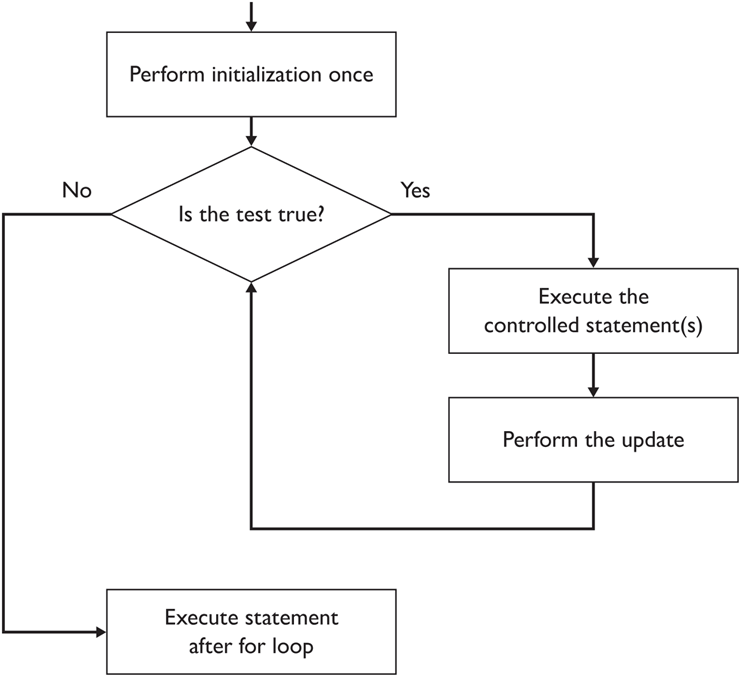
\includegraphics[width=\maxwidth,height=\maxheight,keepaspectratio,alt={Image}]{Figures/img_p69_0.png}}
\end{center}


\caption{Image}
\end{figure}

được thực hiện sau khi các câu lệnh được điều khiển đã được thực thi.
Khi phép kiểm tra đánh giá thành \texttt{false}, Java hoàn thành việc
thực thi vòng lặp và chuyển sang bất kỳ câu lệnh nào đứng sau vòng lặp.

Vòng lặp \texttt{for} là ví dụ đầu tiên về một cấu trúc điều khiển mà
chúng ta sẽ nghiên cứu.

\begin{quote}
\textbf{Cấu trúc điều khiển (Control Structure)} Một cấu trúc cú pháp
điều khiển các câu lệnh khác.
\end{quote}

Bạn nên cẩn thận sử dụng việc thụt lề để chỉ định các câu lệnh được điều
khiển. Trong trường hợp vòng lặp \texttt{for}, tất cả các câu lệnh trong
phần thân của vòng lặp được thụt lề như một cách để chỉ ra rằng chúng
nằm ``bên trong'' vòng lặp.

\subsubsection{\texorpdfstring{Theo Dõi Vòng Lặp \texttt{for} (Tracing
for
Loops)}{Theo Dõi Vòng Lặp for (Tracing for Loops)}}\label{theo-duxf5i-vuxf2ng-lux1eb7p-for-tracing-for-loops}

Hãy kiểm tra chi tiết vòng lặp \texttt{for} của chương trình
\texttt{WriteSquares2}:

\begin{verbatim}
for (int i = 1; i <= 5; i++) {
    System.out.println(i + " squared = " + (i * i));
}
\end{verbatim}

Trong vòng lặp này, phần khởi tạo (\texttt{int\ i\ =\ 1}) khai báo một
biến số nguyên \texttt{i} được khởi tạo bằng \texttt{1}. Phép kiểm tra
tiếp tục (\texttt{i\ \textless{}=\ 5}) chỉ ra rằng chúng ta nên tiếp tục
thực thi chừng nào \texttt{i} còn nhỏ hơn hoặc bằng \texttt{5}. Điều đó
có nghĩa là một khi \texttt{i} lớn hơn \texttt{5}, chúng ta sẽ dừng việc
thực thi phần thân của vòng lặp. Phần cập nhật (\texttt{i++}) sẽ tăng
giá trị của \texttt{i} thêm một mỗi lần, đưa \texttt{i} đến gần hơn với
việc lớn hơn \texttt{5}. Sau năm lần thực thi phần thân và năm lần cập
nhật đi kèm, \texttt{i} sẽ lớn hơn \texttt{5} và vòng lặp sẽ kết thúc
việc thực thi. Hình 2.2 theo dõi quá trình này một cách chi tiết.

\emph{Hình 2.2 Theo dõi chi tiết của vòng lặp \texttt{for}}

Java cho phép sự linh hoạt tuyệt vời trong việc quyết định những gì sẽ
đưa vào phần khởi tạo và phần cập nhật, vì vậy chúng ta có thể sử dụng
vòng lặp \texttt{for} để giải quyết đủ loại nhiệm vụ lập trình. Tuy
nhiên, hiện tại, chúng ta sẽ giới hạn mình trong một loại vòng lặp cụ
thể chuyên khai báo và khởi tạo một biến duy nhất được sử dụng để điều
khiển vòng lặp. Biến này thường được gọi là biến vòng lặp (loop
variable) của vòng lặp. Trong phần kiểm tra, chúng ta so sánh biến vòng
lặp với một số giá trị mong muốn cuối cùng, và trong phần cập nhật,
chúng ta thay đổi giá trị của biến vòng lặp, thường là tăng nó thêm
\texttt{1}. Các vòng lặp như vậy rất phổ biến trong lập trình. Theo quy
ước, chúng ta thường sử dụng các tên như \texttt{i}, \texttt{j}, và
\texttt{k} cho các biến vòng lặp.

\begin{figure}
\centering


\begin{center}
\pandocbounded{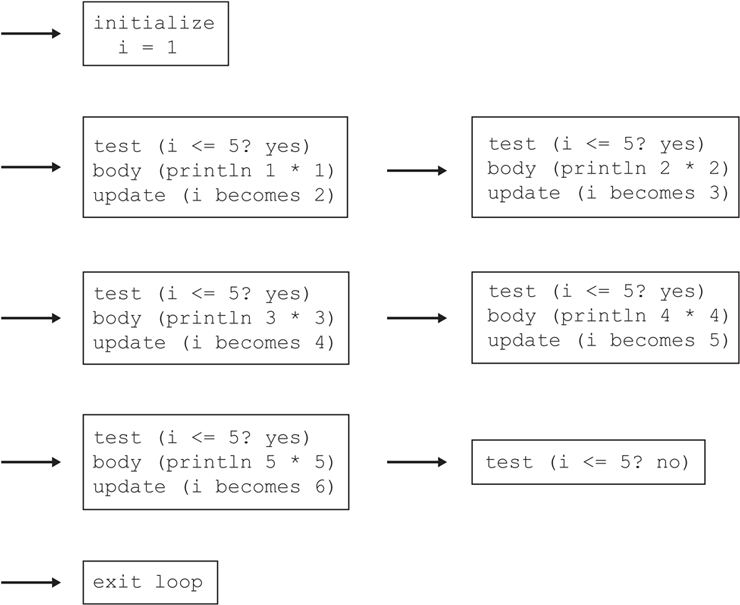
\includegraphics[width=\maxwidth,height=\maxheight,keepaspectratio,alt={Image}]{Figures/img_p72_0.png}}
\end{center}


\caption{Image}
\end{figure}

Mỗi lần thực thi câu lệnh được điều khiển của một vòng lặp được gọi là
một vòng lặp (iteration) của vòng lặp (như trong câu, ``Vòng lặp kết
thúc việc thực thi sau bốn vòng lặp''). Iteration (sự lặp lại) cũng dùng
để chỉ việc lặp nói chung (như trong câu, ``Tôi đã giải quyết bài toán
bằng cách sử dụng iteration'').

Hãy xem xét một vòng lặp \texttt{for} khác:

\begin{verbatim}
for (int i = -100; i <= 100; i++) {
    System.out.println(i + " squared = " + (i * i));
}
\end{verbatim}

Vòng lặp này thực thi tổng cộng \texttt{201} lần, tạo ra bình phương của
tất cả các số nguyên nằm giữa \texttt{-100} và \texttt{+100} bao gồm cả
hai đầu. Do đó, các giá trị được sử dụng trong phần khởi tạo và phần
kiểm tra có thể là bất kỳ số nguyên nào. Trên thực tế, chúng có thể là
các biểu thức số nguyên tùy ý:

\begin{verbatim}
for (int i = (2 + 2); i <= (17 * 3); i++) {
    System.out.println(i + " squared = " + (i * i));
}
\end{verbatim}

Vòng lặp này sẽ tạo ra bình phương của tất cả các số nguyên nằm giữa
\texttt{4} và \texttt{51} bao gồm cả hai đầu. Các dấu ngoặc đơn xung
quanh các biểu thức là không cần thiết nhưng cải thiện khả năng đọc. Hãy
xem xét vòng lặp sau:

\begin{verbatim}
for (int i = 1; i <= 30; i++) {
    System.out.println("+--------+");
}
\end{verbatim}

Vòng lặp này tạo ra \texttt{30} dòng kết quả đầu ra, tất cả đều hoàn
toàn giống nhau. Nó hơi khác so với vòng lặp trước bởi vì câu lệnh được
điều khiển bởi vòng lặp \texttt{for} không liên quan gì đến biến vòng
lặp. Do đó,

\begin{verbatim}
for (int i = -30; i <= -1; i++) {
    System.out.println("+--------+");
}
\end{verbatim}

tạo ra kết quả hoàn toàn giống y hệt. Hành vi của một vòng lặp như vậy
được xác định duy nhất bởi số vòng lặp (iterations) mà nó thực hiện. Số
vòng lặp được cung cấp bởi công thức:
\texttt{\textless{}giá\ trị\ kết\ thúc\textgreater{}\ -\ \textless{}giá\ trị\ bắt\ đầu\textgreater{}\ +\ 1}

Sẽ đơn giản hơn nhiều khi thấy rằng vòng lặp đầu tiên trong số này lặp
\texttt{30} lần, vì vậy tốt hơn là sử dụng vòng lặp đó.

Bây giờ chúng ta hãy xem xét một số trường hợp ranh giới (borderline
cases). Hãy xem xét vòng lặp này:

\begin{verbatim}
for (int i = 1; i <= 1; i++) {
    System.out.println("+--------+");
}
\end{verbatim}

Theo quy tắc của chúng ta, nó sẽ lặp một lần, và thực tế là như vậy. Nó
khởi tạo biến \texttt{i} bằng \texttt{1} và kiểm tra xem biến này có nhỏ
hơn hoặc bằng \texttt{1} hay không, và điều đó là đúng. Vì vậy, nó thực
thi \texttt{println}, tăng \texttt{i}, và kiểm tra lại. Lần thứ hai nó
kiểm tra, nó thấy rằng \texttt{i} không còn nhỏ hơn hoặc bằng \texttt{1}
nữa, vì vậy nó ngừng thực thi. Bây giờ hãy xem xét vòng lặp này:

\begin{verbatim}
for (int i = 1; i <= 0; i++) {
    System.out.println("+--------+"); // never executes
}
\end{verbatim}

Vòng lặp này hoàn toàn không thực hiện vòng lặp nào cả. Nó sẽ không gây
ra lỗi thực thi; nó chỉ là không thực thi phần thân. Nó khởi tạo biến
thành \texttt{1} và kiểm tra xem biến này có nhỏ hơn hoặc bằng
\texttt{0} hay không. Điều đó là sai, vì vậy thay vì thực thi các câu
lệnh trong phần thân, nó dừng lại ngay ở đó.

Khi bạn xây dựng một vòng lặp \texttt{for}, bạn có thể đưa vào nhiều hơn
một câu lệnh bên trong các dấu ngoặc nhọn. Chẳng hạn, hãy xem xét đoạn
mã sau:

\begin{verbatim}
for (int i = 1; i <= 20; i++) {
    System.out.println("Hi!");
    System.out.println("Ho!");
}
\end{verbatim}

Đoạn mã này sẽ tạo ra \texttt{20} cặp dòng, dòng đầu tiên có từ ``Hi!''
trên đó và dòng thứ hai có từ ``Ho!''.

Khi một vòng lặp \texttt{for} điều khiển một câu lệnh duy nhất, bạn
không bắt buộc phải bao gồm các dấu ngoặc nhọn. Các dấu ngoặc nhọn chỉ
được yêu cầu đối với các tình huống như tình huống trước, nơi bạn có
nhiều hơn một câu lệnh mà bạn muốn vòng lặp điều khiển. Tuy nhiên, quy
ước viết mã của Java là luôn bao gồm các dấu ngoặc nhọn ngay cả đối với
một câu lệnh duy nhất, và chúng tôi tuân theo quy ước này trong cuốn
sách này. Có hai ưu điểm đối với quy ước này: - Việc bao gồm các dấu
ngoặc nhọn ngăn ngừa các lỗi trong tương lai. Ngay cả khi bây giờ bạn
chỉ cần một câu lệnh trong phần thân của vòng lặp, mã của bạn có thể sẽ
thay đổi theo thời gian. Việc có sẵn các dấu ngoặc nhọn ở đó đảm bảo
rằng, nếu bạn thêm một câu lệnh bổ sung vào phần thân sau này, bạn sẽ
không vô tình quên bao gồm chúng. Nói chung, việc bao gồm các dấu ngoặc
nhọn trước sẽ đỡ tốn công sức hơn so với việc phải tìm kiếm các lỗi khó
hiểu sau này. - Luôn bao gồm các dấu ngoặc nhọn làm giảm mức độ chi tiết
bạn phải xem xét khi học các cấu trúc điều khiển mới. Sẽ mất thời gian
để làm chủ các chi tiết của bất kỳ cấu trúc điều khiển mới nào, và việc
làm chủ những chi tiết đó sẽ dễ dàng hơn nếu bạn không phải suy nghĩ
thêm về việc khi nào nên bao gồm và khi nào không nên bao gồm các dấu
ngoặc.

\begin{quote}
{[}!WARNING{]} \textbf{LỖI LẬP TRÌNH PHỔ BIẾN} \textbf{Quên Dấu Ngoặc
Nhọn (Forgetting Curly Braces)}

Bạn nên sử dụng việc thụt lề để chỉ định phần thân của một vòng lặp
\texttt{for}, nhưng thụt lề thôi là chưa đủ. Java bỏ qua việc thụt lề
khi quyết định xem các câu lệnh khác nhau được nhóm lại như thế nào.
Chẳng hạn, giả sử bạn viết đoạn mã sau:

\begin{verbatim}
for (int i = 1; i <= 20; i++)
    System.out.println("Hi!");
    System.out.println("Ho!");
\end{verbatim}

Việc thụt lề chỉ ra cho người đọc rằng cả hai câu lệnh \texttt{println}
đều nằm trong phần thân của vòng lặp \texttt{for}, nhưng không có bất kỳ
dấu ngoặc nhọn nào để báo cho Java biết điều đó. Kết quả là, đoạn mã này
được diễn giải như sau:

\begin{verbatim}
for (int i = 1; i <= 20; i++) {
    System.out.println("Hi!");
}
System.out.println("Ho!");
\end{verbatim}

Chỉ câu lệnh \texttt{println} đầu tiên được coi là nằm trong phần thân
của vòng lặp \texttt{for}. Câu lệnh \texttt{println} thứ hai được coi là
nằm bên ngoài vòng lặp. Vì vậy, đoạn mã này sẽ tạo ra \texttt{20} dòng
kết quả đầu ra đều ghi là ``Hi!'' theo sau là một dòng kết quả đầu ra
ghi là ``Ho!''. Để bao gồm cả hai lệnh \texttt{println} vào trong phần
thân, bạn cần các dấu ngoặc nhọn xung quanh chúng:

\begin{verbatim}
for (int i = 1; i <= 20; i++) {
    System.out.println("Hi!");
    System.out.println("Ho!");
}
\end{verbatim}
\end{quote}

\subsubsection{\texorpdfstring{Các Mẫu Vòng Lặp \texttt{for} (for Loop
Patterns)}{Các Mẫu Vòng Lặp for (for Loop Patterns)}}\label{cuxe1c-mux1eabu-vuxf2ng-lux1eb7p-for-for-loop-patterns}

Nói chung, nếu bạn muốn một vòng lặp thực hiện chính xác \(n\) lần lặp,
bạn sẽ sử dụng một trong hai vòng lặp tiêu chuẩn. Dạng tiêu chuẩn đầu
tiên trông giống như những dạng bạn đã thấy:

\begin{verbatim}
for (int <variable> = 1; <variable> <= n; <variable>++) {
    <statement>;
    <statement>;
    ...
    <statement>;
}
\end{verbatim}

Khá rõ ràng là vòng lặp này thực thi \(n\) lần, bởi vì nó bắt đầu ở
\texttt{1} và tiếp tục chừng nào nó còn nhỏ hơn hoặc bằng \(n\). Ví dụ,
vòng lặp này in ra các số từ \texttt{1} đến \texttt{10}:

\begin{verbatim}
for (int i = 1; i <= 10; i++) {
    System.out.print(i + " ");
}
\end{verbatim}

Bởi vì nó sử dụng một câu lệnh \texttt{print} thay vì \texttt{println},
nó tạo ra một dòng kết quả đầu ra duy nhất:

\begin{verbatim}
1 2 3 4 5 6 7 8 9 10
\end{verbatim}

Tuy nhiên, thường thì việc bắt đầu đếm của chúng ta ở số \texttt{0} thay
vì \texttt{1} sẽ thuận tiện hơn. Điều đó đòi hỏi phải có sự thay đổi
trong phần kiểm tra vòng lặp để cho phép bạn dừng lại khi nó nhỏ hơn
\(n\) một đơn vị:

\begin{verbatim}
for (int <variable> = 0; <variable> < n; i++) {
    <statement>;
    <statement>;
    ...
    <statement>;
}
\end{verbatim}

Lưu ý rằng trong dạng này, khi bạn khởi tạo biến thành \texttt{0}, bạn
kiểm tra xem nó có nhỏ hơn một cách nghiêm ngặt so với \(n\) hay không.
Cả hai dạng sẽ thực thi chính xác \(n\) lần, mặc dù có một số tình huống
mà vòng lặp dựa trên số không (zero-based loop) hoạt động tốt hơn. Ví
dụ, vòng lặp này thực thi \texttt{10} lần giống như vòng lặp trước:

\begin{verbatim}
for (int i = 0; i < 10; i++) {
    System.out.print(i + " ");
}
\end{verbatim}

Bởi vì nó bắt đầu ở \texttt{0} thay vì bắt đầu ở \texttt{1}, nó tạo ra
một chuỗi \texttt{10} giá trị khác nhau:

\begin{verbatim}
0 1 2 3 4 5 6 7 8 9
\end{verbatim}

Thông thường nhất, bạn sẽ sử dụng vòng lặp bắt đầu ở \texttt{0} hoặc
\texttt{1} để thực hiện một số thao tác một số lần cố định. Nhưng có một
biến thể nhỏ đôi khi cũng hữu ích. Thay vì chạy vòng lặp theo hướng
tiến, chúng ta có thể chạy nó theo hướng lùi. Thay vì bắt đầu ở
\texttt{1} và thực thi cho đến khi bạn đạt đến \(n\), bạn lại bắt đầu ở
\(n\) và tiếp tục thực thi cho đến khi bạn đạt đến \texttt{1}. Bạn có
thể đạt được điều này bằng cách sử dụng phép giảm (decrement) thay vì
phép tăng (increment), vì vậy đôi khi chúng ta gọi đây là một vòng lặp
giảm (decrementing loop).

Dưới đây là dạng tổng quát của một vòng lặp giảm:

\begin{verbatim}
for (int <variable> = n; <variable> >= 1; <variable>--) {
    <statement>;
    <statement>;
    ...
    <statement>;
}
\end{verbatim}

Ví dụ, dưới đây là một vòng lặp giảm thực thi \texttt{10} lần:

\begin{verbatim}
for (int i = 10; i >= 1; i--) {
    System.out.print(i + " ");
}
\end{verbatim}

Bởi vì nó chạy lùi, nó in ra các giá trị theo thứ tự ngược lại:

\begin{verbatim}
10 9 8 7 6 5 4 3 2 1
\end{verbatim}

JShell cho phép bạn viết các vòng lặp \texttt{for}. Vì một vòng lặp kéo
dài nhiều dòng, shell sẽ hiển thị lời nhắc tiếp tục là
\texttt{...\textgreater{}} trên mỗi dòng tiếp theo cho đến khi bạn kết
thúc vòng lặp bằng cách viết dấu ngoặc nhọn đóng \texttt{\}}, như được
hiển thị trong tương tác sau. Khi bạn viết xong vòng lặp hoàn chỉnh,
vòng lặp sẽ thực thi.

\begin{verbatim}
jshell> for (int i = 1; i <= 10; i++) {
  ...>     System.out.print(i + "! ");
  ...> } 
1! 2! 3! 4! 5! 6! 7! 8! 9! 10!
\end{verbatim}

\subsubsection{\texorpdfstring{Các Vòng Lặp \texttt{for} Lồng Nhau
(Nested for
Loops)}{Các Vòng Lặp for Lồng Nhau (Nested for Loops)}}\label{cuxe1c-vuxf2ng-lux1eb7p-for-lux1ed3ng-nhau-nested-for-loops}

Vòng lặp \texttt{for} điều khiển một câu lệnh, và bản thân vòng lặp
\texttt{for} cũng là một câu lệnh, điều đó có nghĩa là một vòng lặp
\texttt{for} có thể điều khiển một vòng lặp \texttt{for} khác. Ví dụ,
bạn có thể viết đoạn mã như sau:

\begin{verbatim}
for (int i = 1; i <= 10; i++) {
    for (int j = 1; j <= 5; j++) {
        System.out.println("Hi there.");
    }
}
\end{verbatim}

Đoạn mã này có lẽ dễ đọc hơn từ trong ra ngoài. Câu lệnh
\texttt{println} tạo ra một dòng kết quả đầu ra duy nhất. Vòng lặp
\texttt{j} bên trong thực thi câu lệnh này năm lần, tạo ra năm dòng kết
quả đầu ra. Vòng lặp \texttt{i} bên ngoài thực thi vòng lặp bên trong
\texttt{10} lần, tạo ra \texttt{10} tập hợp gồm \texttt{5} dòng, hay
\texttt{50} dòng kết quả đầu ra. Do đó, đoạn mã trước đó tương đương
với:

\begin{verbatim}
for (int i = 1; i <= 50; i++) {
    System.out.println("Hi there.");
}
\end{verbatim}

Ví dụ này cho thấy rằng một vòng lặp \texttt{for} có thể được điều khiển
bởi một vòng lặp \texttt{for} khác. Một vòng lặp như vậy được gọi là một
vòng lặp lồng nhau (nested loop). Tuy nhiên, ví dụ này không thú vị lắm,
bởi vì vòng lặp lồng nhau có thể bị loại bỏ.

Bây giờ bạn đã biết cách viết các vòng lặp \texttt{for}, bạn sẽ muốn có
thể tạo ra các dòng kết quả đầu ra phức tạp từng phần một bằng cách sử
dụng lệnh \texttt{print}. Hãy nhớ lại từ Chương 1 rằng lệnh
\texttt{print} in trên dòng kết quả đầu ra hiện tại mà không chuyển sang
dòng kết quả đầu ra mới. Ví dụ, nếu bạn muốn tạo ra một dòng kết quả đầu
ra có \texttt{80} ngôi sao trên đó, bạn có thể sử dụng một lệnh
\texttt{print} để in từng ngôi sao một và để nó thực thi \texttt{80} lần
thay vì sử dụng một lệnh \texttt{println} duy nhất.

Hãy xem xét một vòng lặp lồng nhau thú vị hơn sử dụng lệnh
\texttt{print}:

\begin{verbatim}
for (int i = 1; i <= 6; i++) {
    for (int j = 1; j <= 3; j++) {
        System.out.print(j + " ");
    }
}
\end{verbatim}

Chúng ta có thể một lần nữa đọc điều này từ trong ra ngoài. Vòng lặp bên
trong in ra giá trị của biến vòng lặp \texttt{j} của nó khi nó thay đổi
từ \texttt{1} đến \texttt{3}. Vòng lặp bên ngoài thực thi điều này sáu
lần khác nhau. Kết quả là, chúng ta nhận được sáu lần xuất hiện của
chuỗi \texttt{1\ 2\ 3} làm kết quả đầu ra:

\begin{verbatim}
1 2 3 1 2 3 1 2 3 1 2 3 1 2 3 1 2 3
\end{verbatim}

Đoạn mã này in tất cả kết quả đầu ra của nó trên một dòng kết quả đầu ra
duy nhất. Hãy xem một số mã bao gồm sự kết hợp của \texttt{print} và
\texttt{println} để tạo ra một số dòng kết quả đầu ra:

\begin{verbatim}
for (int i = 1; i <= 6; i++) {
    for (int j = 1; j <= 10; j++) {
        System.out.print("*");
    }
    System.out.println();
}
\end{verbatim}

Khi bạn viết đoạn mã có liên quan đến các vòng lặp lồng nhau, bạn phải
cẩn thận thụt lề đoạn mã một cách chính xác để làm cho cấu trúc rõ ràng.
Ở cấp độ ngoài cùng, đoạn mã trước đó là một vòng lặp \texttt{for} đơn
giản thực thi sáu lần:

\begin{verbatim}
for (int i = 1; i <= 6; i++) {
    ...
}
\end{verbatim}

Chúng ta sử dụng thụt lề cho các câu lệnh bên trong vòng lặp
\texttt{for} này để làm rõ rằng chúng là phần thân của vòng lặp này. Bên
trong, chúng ta tìm thấy hai câu lệnh: một vòng lặp \texttt{for} khác và
một \texttt{println}. Hãy xem xét vòng lặp \texttt{for} bên trong:

\begin{verbatim}
for (int j = 1; j <= 10; j++) {
    System.out.print("*");
}
\end{verbatim}

Vòng lặp này được điều khiển bởi vòng lặp \texttt{for} bên ngoài, đó là
lý do tại sao nó được thụt lề, nhưng bản thân nó lại điều khiển một câu
lệnh (câu lệnh \texttt{print}), vì vậy chúng ta lại có thêm một cấp độ
thụt lề nữa. Do đó, việc thụt lề chỉ ra rằng câu lệnh \texttt{print}
được điều khiển bởi vòng lặp \texttt{for} bên trong, và vòng lặp này đến
lượt nó lại được điều khiển bởi vòng lặp \texttt{for} bên ngoài. Vậy
vòng lặp bên trong này làm gì? Nó in ra \texttt{10} ngôi sao trên dòng
kết quả đầu ra hiện tại. Chúng đều xuất hiện trên cùng một dòng vì chúng
ta đang sử dụng một lệnh \texttt{print} thay vì \texttt{println}. Lưu ý
rằng sau vòng lặp này, chúng ta thực hiện một lệnh \texttt{println}:

\begin{verbatim}
System.out.println();
\end{verbatim}

Hiệu ứng ròng của vòng lặp \texttt{for} theo sau bởi \texttt{println} là
chúng ta nhận được một dòng kết quả đầu ra với \texttt{10} ngôi sao trên
đó. Nhưng hãy nhớ rằng các câu lệnh này được chứa trong một vòng lặp bên
ngoài thực thi sáu lần, vì vậy cuối cùng chúng ta nhận được sáu dòng kết
quả đầu ra, mỗi dòng có \texttt{10} ngôi sao:

\begin{verbatim}
********** 
********** 
********** 
********** 
********** 
**********
\end{verbatim}

Hãy xem xét thêm một biến thể nữa. Trong đoạn mã trên, vòng lặp
\texttt{for} bên trong luôn thực hiện chính xác một công việc giống
nhau: Nó in chính xác \texttt{10} ngôi sao trên một dòng kết quả đầu ra.
Nhưng điều gì sẽ xảy ra nếu chúng ta thay đổi phép kiểm tra cho vòng lặp
\texttt{for} bên trong để sử dụng biến (\texttt{i}) của vòng lặp
\texttt{for} bên ngoài?

\begin{verbatim}
for (int i = 1; i <= 6; i++) {
    for (int j = 1; j <= i; j++) {
        System.out.print("*");
    }
    System.out.println();
}
\end{verbatim}

Trong phiên bản cũ, vòng lặp bên trong luôn thực thi \texttt{10} lần,
tạo ra \texttt{10} ngôi sao trên mỗi dòng kết quả đầu ra. Với phép kiểm
tra mới (\texttt{j\ \textless{}=\ i}), vòng lặp bên trong sẽ thực thi
\texttt{i} lần với mỗi lần lặp. Nhưng \texttt{i} đang thay đổi: Nó nhận
các giá trị \texttt{1}, \texttt{2}, \texttt{3}, \texttt{4}, \texttt{5},
và \texttt{6}. Ở lần lặp đầu tiên của vòng lặp bên ngoài, khi \texttt{i}
là \texttt{1}, phép kiểm tra \texttt{j\ \textless{}=\ i} thực chất là
đang kiểm tra \texttt{j\ \textless{}=\ 1}, và nó tạo ra một dòng có một
ngôi sao trên đó. Ở lần lặp thứ hai của vòng lặp bên ngoài, khi
\texttt{i} là \texttt{2}, phép kiểm tra thực chất là đang kiểm tra
\texttt{j\ \textless{}=\ 2}, và nó tạo ra một dòng có hai ngôi sao trên
đó. Ở lần lặp thứ ba của vòng lặp bên ngoài, khi \texttt{i} là
\texttt{3}, phép kiểm tra thực chất là đang kiểm tra
\texttt{j\ \textless{}=\ 3}, và nó tạo ra một dòng có ba ngôi sao trên
đó. Quá trình này tiếp tục qua lần lặp thứ sáu.

Nói cách khác, đoạn mã này tạo ra một hình tam giác làm kết quả đầu ra:

\begin{verbatim}
* 
** 
*** 
**** 
***** 
******
\end{verbatim}

\subsection{Quản Lý Độ Phức Tạp (Managing
Complexity)}\label{quux1ea3n-luxfd-ux111ux1ed9-phux1ee9c-tux1ea1p-managing-complexity}

Bạn đã học về một số cấu trúc lập trình mới trong chương này, và đã đến
lúc kết hợp các mảnh ghép lại với nhau để giải quyết một số nhiệm vụ
phức tạp. Như chúng tôi đã chỉ ra trong Chương 1, Brian Kernighan, một
trong những đồng tác giả của cuốn \emph{The C Programming Language}, đã
nói rằng ``Kiểm soát độ phức tạp là bản chất của lập trình máy tính''
(``Controlling complexity is the essence of computer programming'').
Trong phần này, chúng ta sẽ xem xét một số kỹ thuật mà các nhà khoa học
máy tính sử dụng để giải quyết các vấn đề phức tạp mà không bị choáng
ngợp bởi độ phức tạp.

\subsubsection{Phạm Vi (Scope)}\label{phux1ea1m-vi-scope}

Khi các chương trình trở nên dài hơn, khả năng các phần khác nhau của
chương trình can thiệp lẫn nhau ngày càng tăng. Java giúp chúng ta quản
lý vấn đề tiềm ẩn này bằng cách thực thi các quy tắc về phạm vi.

\begin{quote}
\textbf{Phạm vi (Scope)} Phần của một chương trình mà tại đó một khai
báo cụ thể có giá trị hợp lệ.
\end{quote}

Như bạn đã thấy, khi nói đến việc khai báo các phương thức tĩnh (static
methods), bạn có thể đặt chúng theo bất kỳ thứ tự nào. Phạm vi của một
phương thức tĩnh là toàn bộ lớp mà nó xuất hiện. Các biến lại hoạt động
khác. Quy tắc đơn giản là phạm vi của một khai báo biến mở rộng từ điểm
mà nó được khai báo đến dấu ngoặc nhọn đóng \texttt{\}} bao bọc nó. Nói
cách khác, hãy tìm cặp dấu ngoặc nhọn trực tiếp bao bọc khai báo biến.
Phạm vi của biến là từ điểm nó được khai báo đến dấu ngoặc nhọn đóng.

Quy tắc phạm vi này có một số hàm ý. Đầu tiên, hãy xem xét nó có ý nghĩa
gì đối với các phương thức khác nhau. Mỗi phương thức có tập hợp các dấu
ngoặc nhọn riêng để chỉ định các câu lệnh sẽ được thực thi khi phương
thức được gọi. Bất kỳ biến nào được khai báo bên trong các dấu ngoặc
nhọn của một phương thức sẽ không có sẵn ở bên ngoài phương thức đó.
Chúng ta gọi các biến như vậy là các biến cục bộ (local variables), và
chúng ta gọi quá trình giới hạn phạm vi của chúng là cục bộ hóa các biến
(localizing variables).

\begin{quote}
\textbf{Biến cục bộ (Local Variable)} Một biến được khai báo bên trong
một phương thức, chỉ có thể truy cập được trong phương thức đó.
\end{quote}

\begin{quote}
\textbf{Cục bộ hóa các biến (Localizing Variables)} Khai báo các biến
trong phạm vi cục bộ nhất (trong cùng nhất) có thể.
\end{quote}

Nói chung, bạn sẽ muốn khai báo các biến trong phạm vi cục bộ nhất có
thể. Bạn có thể tự hỏi tại sao chúng ta lại muốn cục bộ hóa các biến chỉ
trong một phương thức. Tại sao không khai báo tất cả mọi thứ trong một
phạm vi bên ngoài duy nhất? Điều đó chắc chắn có vẻ đơn giản hơn, nhưng
có một số nhược điểm quan trọng. Việc cục bộ hóa các biến dẫn đến một số
sự trùng lặp (và có thể gây nhầm lẫn) nhưng cung cấp bảo mật tốt hơn. Để
so sánh, hãy xem xét việc sử dụng tủ lạnh trong các ký túc xá. Mỗi phòng
ký túc xá có thể có tủ lạnh riêng, nhưng nếu bạn ở bên ngoài một phòng,
bạn không biết liệu nó có tủ lạnh bên trong hay không. Nội dung của căn
phòng được giấu kín khỏi bạn.

Các chương trình Java sử dụng các biến để lưu trữ các giá trị giống như
sinh viên sử dụng tủ lạnh để lưu trữ bia, kem và những thứ có giá trị
khác. Lần cuối cùng chúng tôi ở trong một ký túc xá, chúng tôi nhận thấy
rằng hầu hết các phòng cá nhân đều có tủ lạnh bên trong. Điều này có vẻ
cực kỳ dư thừa, nhưng lý do thì quá rõ ràng. Nếu bạn muốn đảm bảo an
toàn cho một thứ gì đó, bạn đặt nó ở nơi mà không ai khác có thể lấy
được. Bạn sẽ sử dụng các biến cục bộ trong các chương trình của mình
theo cách rất giống như vậy. Nếu mỗi phương thức riêng lẻ có các biến
cục bộ riêng để sử dụng, bạn không phải xem xét khả năng can thiệp từ
các phần khác của chương trình.

Hãy xem xét một ví dụ đơn giản liên quan đến hai phương thức:

\begin{verbatim}
 1  // This program does not compile.
 2  public class ScopeExample {
 3      public static void main(String[] args) {
 4          int x = 3;
 5          int y = 7;
 6          computeSum();
 7      }
 8
 9      public static void computeSum() {
10          int sum = x + y; // illegal, x/y are not in scope
11          System.out.println("sum = " + sum);
12      }
13  }
\end{verbatim}

Trong ví dụ này, phương thức \texttt{main} khai báo các biến cục bộ
\texttt{x} và \texttt{y} và cung cấp cho chúng các giá trị khởi tạo. Sau
đó, nó gọi phương thức \texttt{computeSum}. Bên trong phương thức này,
chúng ta cố gắng sử dụng các giá trị của \texttt{x} và \texttt{y} để
tính tổng. Tuy nhiên, vì các biến \texttt{x} và \texttt{y} là cục bộ đối
với phương thức \texttt{main} và không hiển thị bên trong phương thức
\texttt{computeSum}, điều này không hoạt động. (Trong chương tiếp theo,
chúng ta sẽ thấy một kỹ thuật cho phép một phương thức truyền một giá
trị cho phương thức khác.)

Chương trình tạo ra các thông báo lỗi giống như sau:

\begin{verbatim}
ScopeExample.java:10: error: cannot find symbol
symbol  : variable x
location: class ScopeExample
        int sum = x + y;  // illegal, x/y are not in scope
                  ^
ScopeExample.java:10: error: cannot find symbol
symbol  : variable y
location: class ScopeExample
        int sum = x + y;  // illegal, x/y are not in scope
                      ^
\end{verbatim}

Việc hiểu phạm vi trong việc thảo luận về các biến cục bộ của phương
thức này so với phương thức khác là rất quan trọng. Phạm vi cũng có hàm
ý đối với những gì xảy ra bên trong một phương thức duy nhất. Bạn đã
thấy rằng các dấu ngoặc nhọn được sử dụng để nhóm một loạt các câu lệnh
lại với nhau. Nhưng bạn có thể có các dấu ngoặc nhọn bên trong các dấu
ngoặc nhọn, và điều này dẫn đến một số vấn đề về phạm vi. Ví dụ, hãy xem
xét đoạn mã sau:

\begin{verbatim}
for (int i = 1; i <= 5; i++) {
    int squared = i * i;
    System.out.println(i + " squared = " + squared);
}
\end{verbatim}

Đây là một biến thể của đoạn mã mà chúng ta đã xem xét trước đó trong
chương để in ra bình phương của năm số nguyên đầu tiên. Trong phiên bản
này, một biến được gọi là \texttt{squared} được sử dụng để theo dõi bình
phương của biến vòng lặp \texttt{for}. Đoạn mã này hoạt động tốt, nhưng
hãy xem xét biến thể này:

\begin{verbatim}
for (int i = 1; i <= 5; i++) {
    int squared = i * i;
    System.out.println(i + " squared = " + squared);
}
System.out.println("Last square = " + squared); // illegal
\end{verbatim}

Đoạn mã này tạo ra một lỗi trình biên dịch. Biến \texttt{squared} được
khai báo bên trong vòng lặp \texttt{for}. Nói cách khác, các dấu ngoặc
nhọn chứa nó là các dấu ngoặc nhọn của vòng lặp. Nó không thể được sử
dụng bên ngoài phạm vi này, vì vậy khi bạn cố gắng tham chiếu đến nó bên
ngoài vòng lặp, bạn sẽ nhận được lỗi biên dịch.

Nếu vì lý do nào đó bạn cần viết mã như thế này để truy cập biến sau
vòng lặp, bạn phải khai báo biến trong phạm vi bên ngoài, trước vòng
lặp:

\begin{verbatim}
int squared = 0;   // declaration is now in outer scope
for (int i = 1; i <= 5; i++) {
    squared = i * i;   // change this to an assignment statement
    System.out.println(i + " squared = " + squared);
}
System.out.println("Last square = " + squared); // now legal
\end{verbatim}

Có một vài trường hợp đặc biệt đối với phạm vi, và vòng lặp \texttt{for}
là một trong số đó. Khi một biến được khai báo trong phần khởi tạo của
một vòng lặp \texttt{for}, phạm vi của nó chỉ là bản thân vòng lặp
\texttt{for} (ba phần trong tiêu đề vòng lặp \texttt{for} và các câu
lệnh được điều khiển bởi vòng lặp \texttt{for}). Điều đó có nghĩa là bạn
có thể sử dụng cùng một tên biến trong nhiều vòng lặp \texttt{for}:

\begin{verbatim}
for (int i = 1; i <= 10; i++) {
    System.out.println(i + " squared = " + (i * i));
}
for (int i = 1; i <= 10; i++) {
    System.out.println(i + " cubed = " + (i * i * i));
}
\end{verbatim}

Biến \texttt{i} được khai báo hai lần trong đoạn mã trước đó, nhưng vì
phạm vi của mỗi biến chỉ là vòng lặp \texttt{for} mà nó được khai báo,
nên đây không phải là vấn đề. (Điều này giống như việc có hai phòng ký
túc xá, mỗi phòng đều có tủ lạnh riêng.) Tất nhiên, bạn không thể làm
điều này với các vòng lặp \texttt{for} lồng nhau. Chẳng hạn, đoạn mã sau
sẽ không biên dịch được:

\begin{verbatim}
for (int i = 1; i <= 5; i++) {
    for (int i = 1; i <= 10; i++) { // illegal
        System.out.println("hi there.");
    }
}
\end{verbatim}

Khi Java gặp vòng lặp \texttt{for} bên trong, nó sẽ phàn nàn rằng biến
\texttt{i} đã được khai báo trong phạm vi này. Bạn không thể khai báo
cùng một biến hai lần trong cùng một phạm vi. Bạn phải đưa ra hai tên
khác nhau để phân biệt chúng, giống như khi có hai người tên Carl trong
cùng một gia đình, họ có xu hướng được gọi là ``Carl con'' và ``Carl
bố'' để tránh bất kỳ sự nhầm lẫn tiềm ẩn nào.

Một biến vòng lặp được sử dụng trong vòng lặp \texttt{for} không nhất
thiết phải được khai báo trong phần khởi tạo của vòng lặp. Bạn có thể
tách việc khai báo biến vòng lặp \texttt{for} khỏi việc khởi tạo biến,
như trong đoạn mã sau:

\begin{verbatim}
int i;
for (i = 1; i <= 5; i++) {
    System.out.println(i + " squared = " + (i * i));
}
\end{verbatim}

Làm như vậy sẽ mở rộng phạm vi của biến đến cuối tập hợp dấu ngoặc nhọn
bao bọc. Một ưu điểm của phương pháp này là nó cho phép bạn tham chiếu
đến giá trị cuối cùng của biến vòng lặp sau vòng lặp. Thông thường bạn
sẽ không thể làm điều này, bởi vì phạm vi của biến vòng lặp sẽ bị giới
hạn ở chính vòng lặp đó. Tuy nhiên, việc khai báo biến vòng lặp bên
ngoài vòng lặp là một thói quen nguy hiểm, và nó cung cấp một ví dụ tốt
về các vấn đề bạn có thể gặp phải khi bạn không cục bộ hóa các biến.
Chẳng hạn, hãy xem xét đoạn mã sau:

\begin{verbatim}
int i;
for (i = 1; i <= 5; i++) {
    for (i = 1; i <= 10; i++) {
        System.out.println("hi there.");
    }
}
\end{verbatim}

Như đã lưu ý ở trên, bạn không nên sử dụng cùng một biến vòng lặp khi
bạn có các vòng lặp lồng nhau. Nhưng không giống như ví dụ trước, đoạn
mã này biên dịch được, bởi vì ở đây khai báo biến nằm ngoài vòng lặp
\texttt{for} bên ngoài. Vì vậy, thay vì nhận được một thông báo lỗi hữu
ích từ trình biên dịch Java, bạn nhận được một chương trình có lỗi (bug)
trong đó. Từ việc đọc các vòng lặp này, bạn có thể nghĩ rằng đoạn mã sẽ
tạo ra \texttt{50} dòng kết quả đầu ra, nhưng thực tế nó chỉ tạo ra
\texttt{10} dòng kết quả đầu ra. Vòng lặp bên trong tăng biến \texttt{i}
cho đến khi nó trở thành \texttt{11}, và điều đó khiến vòng lặp bên
ngoài chấm dứt chỉ sau một lần lặp. Sẽ còn tồi tệ hơn nếu bạn đảo ngược
thứ tự của các vòng lặp này:

\begin{verbatim}
int i;
for (i = 1; i <= 10; i++) {
    for (i = 1; i <= 5; i++) {
        System.out.println("hi there.");
    }
}
\end{verbatim}

Đoạn mã này có một vòng lặp vô hạn (infinite loop).

\begin{quote}
\textbf{Vòng lặp vô hạn (Infinite Loop)} Một vòng lặp không bao giờ kết
thúc.
\end{quote}

Vòng lặp này là vô hạn bởi vì bất kể vòng lặp bên ngoài làm gì với biến
\texttt{i}, vòng lặp bên trong luôn đặt nó trở lại \texttt{1} và lặp cho
đến khi nó trở thành \texttt{6}. Vòng lặp bên ngoài sau đó tăng biến lên
\texttt{7} và thấy rằng \texttt{7} nhỏ hơn hoặc bằng \texttt{10}, vì vậy
nó luôn quay trở lại vòng lặp bên trong, vòng lặp bên trong một lần nữa
lại đặt biến trở lại \texttt{1} và lặp cho đến \texttt{6}. Quá trình này
diễn ra vô tận. Đây là những loại vấn đề can thiệp mà bạn có thể gặp
phải khi không cục bộ hóa các biến.

\begin{quote}
{[}!WARNING{]} \textbf{LỖI LẬP TRÌNH PHỔ BIẾN} \textbf{Tham Chiếu Sai
Biến Vòng Lặp (Referring to the Wrong Loop Variable)}

Đoạn mã sau được dự định để in ra một hình tam giác các ngôi sao. Tuy
nhiên, nó có một lỗi tinh vi khiến nó in ra các ngôi sao vô hạn:

\begin{verbatim}
for (int i = 1; i <= 6; i++) {
    for (int j = 1; j <= i; i++){
        System.out.print("*");
    }
    System.out.println();
}
\end{verbatim}

Vấn đề nằm ở dòng thứ hai, trong câu lệnh cập nhật ở tiêu đề của vòng
lặp \texttt{for} bên trong. Lập trình viên định viết \texttt{j++} nhưng
thay vào đó lại vô tình viết \texttt{i++}. Một dấu vết của đoạn mã được
hiển thị trong Bảng 2.6.

\emph{Bảng 2.6 Dấu vết của vòng lặp \texttt{for} lồng nhau}

Biến \texttt{j} đáng lẽ ra phải tăng lên, nhưng thay vào đó \texttt{i}
lại tăng. Hậu quả của lỗi này là biến \texttt{j} không bao giờ được tăng
trong vòng lặp bên trong, và do đó phép kiểm tra
\texttt{j\ \textless{}=\ i} không bao giờ thất bại, vì vậy vòng lặp bên
trong không kết thúc. Dưới đây là một đoạn mã bị hỏng khác. Đoạn mã này
cố gắng in một hộp các ngôi sao kích thước \texttt{6\ x\ 4}, nhưng nó
cũng in vô hạn:

\begin{verbatim}
for (int i = 1; i <= 6; i++) {
    for (int j = 1; i <= 4; j++) {
        System.out.print("*");
    }
\end{verbatim}
\end{quote}

\begin{verbatim}
    System.out.println();
}
\end{verbatim}

Vấn đề nằm ở dòng thứ hai, lần này là trong phép kiểm tra ở tiêu đề của
vòng lặp \texttt{for} bên trong. Lập trình viên định viết
\texttt{j\ \textless{}=\ 4} nhưng thay vào đó lại vô tình viết
\texttt{i\ \textless{}=\ 4}. Vì giá trị của \texttt{i} không bao giờ
được tăng lên trong vòng lặp bên trong, phép kiểm tra
\texttt{i\ \textless{}=\ 4} không bao giờ thất bại, vì vậy vòng lặp bên
trong lại không kết thúc.

\subsubsection{Mã giả (Pseudocode)}\label{muxe3-giux1ea3-pseudocode}

Khi bạn viết các thuật toán phức tạp hơn, bạn sẽ thấy rằng bạn không thể
chỉ viết toàn bộ thuật toán ngay lập tức. Thay vào đó, bạn sẽ ngày càng
tận dụng kỹ thuật viết mã giả (pseudocode).

\begin{quote}
\textbf{Mã giả (Pseudocode)} Các mô tả bằng tiếng Anh (hoặc ngôn ngữ tự
nhiên) về các thuật toán. Lập trình với mã giả liên quan đến việc tinh
chỉnh liên tiếp một mô tả không chính thức cho đến khi nó dễ dàng được
dịch sang ngôn ngữ Java.
\end{quote}

Ví dụ, bạn có thể mô tả bài toán vẽ một cái hộp như sau: \textgreater{}
\emph{vẽ một cái hộp với \texttt{50} dòng và \texttt{30} cột các dấu hoa
thị.}

Mặc dù câu lệnh này mô tả hình dạng, nó không đưa ra các hướng dẫn cụ
thể về cách vẽ nó (nghĩa là sử dụng thuật toán nào). Bạn vẽ hình theo
từng dòng hay theo từng cột? Trong Java, các hình như thế này phải được
tạo ra theo từng dòng, bởi vì một khi lệnh \texttt{println} đã được thực
hiện trên một dòng kết quả đầu ra, dòng đó không thể bị thay đổi. Không
có lệnh nào để quay trở lại một dòng trước đó trong kết quả đầu ra. Do
đó, bạn phải xuất toàn bộ dòng đầu tiên, rồi đến toàn bộ dòng thứ hai,
và cứ tiếp tục như vậy. Kết quả là, các phân tách (decompositions) của
bạn cho các hình dạng như thế này sẽ định hướng theo dòng
(line-oriented) ở cấp độ trên cùng. Do đó, một phiên bản của câu lệnh
gần với Java hơn là: \textgreater{} \emph{for (mỗi dòng trong số
\texttt{50} dòng) \{} \textgreater{} \emph{vẽ một dòng gồm \texttt{30}
dấu hoa thị.} \textgreater{} \emph{\}}

Hướng dẫn này có thể được cụ thể hóa hơn bằng cách giới thiệu ý tưởng
viết lặp đi lặp lại một ký tự duy nhất trên dòng kết quả đầu ra và sau
đó chuyển sang một dòng kết quả đầu ra mới: \textgreater{} \emph{for
(mỗi dòng trong số \texttt{50} dòng) \{} \textgreater{} \emph{for (mỗi
cột trong số \texttt{30} cột) \{} \textgreater{} \emph{viết một dấu hoa
thị trên dòng kết quả đầu ra.} \textgreater{} \emph{\}} \textgreater{}
\emph{chuyển sang một dòng kết quả đầu ra mới.} \textgreater{} \emph{\}}

Sử dụng mã giả, bạn có thể dần dần chuyển đổi một mô tả bằng tiếng Anh
thành một cái gì đó dễ dàng dịch sang một chương trình Java. Các ví dụ
đơn giản mà chúng ta đã xem xét cho đến nay hầu như không đáng để áp
dụng mã giả, vì vậy bây giờ chúng ta sẽ xem xét bài toán tạo ra một hình
phức tạp hơn:

\begin{verbatim}
********* 
 ******* 
  ***** 
   *** 
    *
\end{verbatim}

Hình này cũng phải được tạo ra theo từng dòng: \textgreater{} \emph{for
(mỗi dòng trong số \texttt{5} dòng) \{} \textgreater{} \emph{vẽ một dòng
của hình tam giác.} \textgreater{} \emph{\}}

Thật không may, mỗi dòng lại khác nhau. Do đó, bạn phải đưa ra một quy
tắc tổng quát phù hợp với tất cả các dòng. Dòng đầu tiên của hình này có
một chuỗi các dấu hoa thị trên đó mà không có khoảng trắng dẫn đầu. Mỗi
dòng tiếp theo có một chuỗi các khoảng trắng theo sau là một chuỗi các
dấu hoa thị. Sử dụng trí tưởng tượng của bạn một chút, bạn có thể nói
rằng dòng đầu tiên có \texttt{0} khoảng trắng trên đó theo sau là một
chuỗi các dấu hoa thị. Điều này cho phép bạn viết một quy tắc tổng quát
để tạo ra hình này: \textgreater{} \emph{for (mỗi dòng trong số
\texttt{5} dòng) \{} \textgreater{} \emph{viết một số khoảng trắng (có
thể là \texttt{0}) trên dòng kết quả đầu ra.} \textgreater{} \emph{viết
một số dấu hoa thị trên dòng kết quả đầu ra.} \textgreater{}
\emph{chuyển sang một dòng kết quả đầu ra mới.} \textgreater{} \emph{\}}

Để tiến hành, bạn phải xác định một quy tắc cho số lượng khoảng trắng và
một quy tắc cho số lượng dấu hoa thị. Bạn muốn tìm một mối quan hệ giữa
số thứ tự của dòng và hai giá trị kia. Đây là đại số đơn giản, bởi vì
các giá trị liên quan với nhau theo cách tuyến tính. Bạn thường cần tìm
ra các biểu thức cho các loại quan hệ tuyến tính này, vì vậy thật đáng
để khám phá một kỹ thuật chung để làm điều đó trước khi chúng ta hoàn
thành mã giả này.

\subsubsection{Kỹ Thuật Lập Bảng (The Table
Technique)}\label{kux1ef9-thuux1eadt-lux1eadp-bux1ea3ng-the-table-technique}

Bạn có thể nhớ lại từ lớp đại số rằng các mối quan hệ tuyến tính được
biểu diễn bằng cách sử dụng một độ dốc (slope) và một tung độ gốc
(intercept). Đối với mục đích của chúng ta, việc coi hai giá trị này là
một hệ số nhân (multiplier) và một hằng số (constant) sẽ dễ dàng hơn.
Chẳng hạn, hãy xem xét các cột giá trị trong Bảng 2.7, đại diện cho số
lượng ký tự trên mỗi dòng cho một hình giả định.

\emph{Bảng 2.7 Đếm Số Ký Tự}

Đối với các chương trình vẽ hình trong chương này, bạn thường có một
vòng lặp \texttt{for} bên ngoài tạo ra kết quả đầu ra theo từng dòng. Do
đó, bạn có xu hướng có một biến gọi là \texttt{line} mang các giá trị
tuần tự bắt đầu từ \texttt{1}, như trong cột đầu tiên của bảng. Nhiệm vụ
của bạn là đưa ra các biểu thức dự đoán các cột số khác.

Có hai bước liên quan đến việc xác định một biểu thức thích hợp cho một
cột số: - Đầu tiên, chọn một hệ số nhân thích hợp bằng cách xem xét các
giá trị tăng hoặc giảm bao nhiêu từ hàng này sang hàng tiếp theo trong
cột đó. - Sau đó, chọn một hằng số thích hợp để cộng vào biểu thức để
tạo ra chuỗi giá trị chính xác.

Hãy nhìn vào cột có nhãn \texttt{value1}. Chú ý rằng các giá trị tăng
lên \texttt{4} mỗi lần khi bạn đi từ hàng này sang hàng tiếp theo. Nếu
bạn định sử dụng biến \texttt{line}, biến này tăng lên \texttt{1} mỗi
lần, để tạo ra các số tăng lên \texttt{4} mỗi lần, bạn sẽ cần nhân nó
với \texttt{4}. Vậy áp dụng bước đầu tiên, bạn sẽ kết thúc với biểu thức
\texttt{(4\ *\ line)}. Nhưng biểu thức này là chưa đủ. Khi \texttt{line}
là \texttt{1}, \texttt{(4\ *\ line)} là \texttt{4} trong khi bạn muốn có
được giá trị \texttt{6}. Bạn sửa điều này ở bước thứ hai.

Bạn cần cộng giá trị nào vào \texttt{4} để có được giá trị \texttt{6}?
Câu trả lời là \texttt{2}. Vì vậy, biểu thức chính xác cần sử dụng là
\texttt{(4\ *\ line\ +\ 2)}. Bạn có thể cắm các giá trị khác nhau của
\texttt{line} vào để xác minh rằng biểu thức này đánh giá thành
\texttt{6} khi \texttt{line} là \texttt{1}, thành \texttt{10} khi
\texttt{line} là \texttt{2}, thành \texttt{14} khi \texttt{line} là
\texttt{3}, và cứ tiếp tục như vậy.

Nếu bạn nhìn vào cột có nhãn \texttt{value2}, bạn sẽ thấy rằng các số
tăng lên \texttt{3} mỗi lần, có nghĩa là bạn muốn một hệ số nhân là
\texttt{3}. Điều đó dẫn đến biểu thức \texttt{(3\ *\ line)}. Ở bước thứ
hai, bạn được cho là phải chọn một hằng số thích hợp để cộng vào biểu
thức này để làm cho nó hoạt động, nhưng biểu thức đã hoạt động, tạo ra
\texttt{3} khi \texttt{line} là \texttt{1}, \texttt{6} khi \texttt{line}
là \texttt{2}, v.v. Đây là một trường hợp đặc biệt nơi hằng số đơn giản
chỉ là \texttt{0} bởi vì không cần điều chỉnh nào khi bạn đã chọn một hệ
số nhân thích hợp.

Các giá trị không phải lúc nào cũng tăng lên. Trong cột có nhãn
\texttt{value3}, bạn sẽ nhận thấy rằng các giá trị giảm đi \texttt{2}
mỗi lần, có nghĩa là bạn muốn một hệ số nhân là \texttt{-2}. Điều đó dẫn
đến biểu thức \texttt{(-2\ *\ line)}. Khi \texttt{line} là \texttt{1},
biểu thức này sẽ đánh giá thành \texttt{-2} trong khi bạn muốn có được
giá trị \texttt{10}. Điều đó có nghĩa là bạn cần cộng thêm \texttt{12}
vào biểu thức, thu được \texttt{(-2\ *\ line\ +\ 12)}. Nhiều lập trình
viên sẽ sắp xếp lại điều này thành \texttt{(12\ -\ 2\ *\ line)}, nhưng
biểu thức nào cũng hoạt động tốt.

Các giá trị trong cột có nhãn \texttt{value4} giảm đi \texttt{1} mỗi
lần, có nghĩa là bạn cần một hệ số nhân là \texttt{-1}. Điều đó dẫn đến
biểu thức \texttt{(-1\ *\ line)}. Biểu thức này đánh giá thành
\texttt{-1} khi \texttt{line} là \texttt{1} trong khi bạn muốn thu được
giá trị \texttt{4}. Điều đó có nghĩa là bạn cần cộng thêm \texttt{5} vào
biểu thức dẫn đến \texttt{(-1\ *\ line\ +\ 5)}. Một lần nữa, hầu hết các
lập trình viên sẽ sắp xếp lại để đơn giản hóa điều này thành
\texttt{(5\ -\ line)}, nhưng cả hai phiên bản của biểu thức đều hoạt
động.

Để áp dụng kỹ thuật này vào bài toán lập trình vẽ hình nón
(cone-drawing) mà chúng ta đang thực hiện trong phần trước, trước tiên
chúng ta lập một bảng có các cột cho số lượng khoảng trắng và dấu hoa
thị mà chúng ta có trên mỗi dòng của kết quả đầu ra. Các giá trị này
được bao gồm trong Bảng 2.8.

\emph{Bảng 2.8 Phân tích hình vẽ}

Chú ý rằng các giá trị trong cột có nhãn \texttt{spaces} tăng lên
\texttt{1} mỗi lần, có nghĩa là bạn muốn một hệ số nhân là \texttt{1}.
Nhưng bạn muốn \texttt{0} khoảng trắng khi \texttt{line} là \texttt{1},
có nghĩa là bạn cần cộng giá trị \texttt{-1} vào biểu thức. Điều đó tạo
ra biểu thức \texttt{(1\ *\ line\ -\ 1)}, hoặc đơn giản là
\texttt{(line\ -\ 1)}.

Các giá trị trong cột có nhãn \texttt{asterisks} giảm đi \texttt{2} mỗi
lần, có nghĩa là chúng ta muốn một hệ số nhân là \texttt{-2}. Điều đó sẽ
tạo ra \texttt{-2} khi \texttt{line} là \texttt{1} trong khi chúng ta
muốn có giá trị \texttt{9}, có nghĩa là chúng ta cần cộng một hằng số là
\texttt{11}. Điều đó tạo ra biểu thức \texttt{(-2\ *\ line\ +\ 11)} hoặc
\texttt{(11\ -\ 2\ *\ line)}.

Sử dụng các biểu thức này, chúng ta có thể cải thiện mã giả của mình như
sau: \textgreater{} \emph{for (line đi từ 1 đến 5) \{} \textgreater{}
\emph{viết (line - 1) khoảng trắng trên dòng kết quả đầu ra.}
\textgreater{} \emph{viết (11 - 2 } line) dấu hoa thị trên dòng kết quả
đầu ra.\emph{ \textgreater{} }chuyển sang một dòng kết quả đầu ra
mới.\emph{ \textgreater{} }\}*

Mã giả này rất đơn giản để biến thành một chương trình:

\begin{verbatim}
 1  // Uses nested loops to draw a 'V' text figure.
 2  public class DrawV {
 3      public static void main(String[] args) {
 4          for (int line = 1; line <= 5; line++) {
 5               for (int i = 1; i <= (line - 1); i++) {
 6                   System.out.print(" ");
 7               }
 8                for (int i = 1; i <= (11 - 2 * line); i++) {
 9                   System.out.print("*");
 10               }
 11                System.out.println();
 12          }
 13      }
 14  }
\end{verbatim}

Đôi khi chúng ta quản lý độ phức tạp bằng cách tận dụng những công việc
mà chúng ta đã làm. Chẳng hạn, làm thế nào bạn tạo ra hình này?

\begin{verbatim}
    * 
   *** 
  ***** 
 ******* 
*********
\end{verbatim}

Bạn có thể làm theo cùng một quy trình như trước đây và tìm các biểu
thức mới để tạo ra số lượng khoảng trắng và dấu hoa thị thích hợp. Tuy
nhiên, có một cách dễ dàng hơn. Hình này giống hình trước, ngoại trừ các
dòng xuất hiện theo thứ tự ngược lại. Đây là một nơi tốt để sử dụng vòng
lặp giảm (decrementing loop) để chạy vòng lặp \texttt{for} ngược lại:
Thay vì bắt đầu từ \texttt{1} và đi lên \texttt{5} với một phép cập nhật
\texttt{++}, bạn có thể bắt đầu từ \texttt{5} và đi xuống \texttt{1}
bằng cách sử dụng một phép cập nhật \texttt{-\/-}. Cách đơn giản để tạo
ra hình tam giác hướng lên trên, do đó, là với đoạn mã sau:

\begin{verbatim}
 1  // Uses nested loops to draw a triangular cone.
 2  public class DrawCone {
 3      public static void main(String[] args) {
 4          for (int line = 5; line >= 1; line--) {
 5              for (int i = 1; i <= (line - 1); i++) {
 6                  System.out.print(" ");
 7              }
 8              for (int i = 1; i <= (11 - 2 * line); i++) {
 9                  System.out.print("*");
 10              }
 11              System.out.println();
 12          }
 13      }
 14  }
\end{verbatim}

\subsubsection{Hằng Số Lớp (Class
Constants)}\label{hux1eb1ng-sux1ed1-lux1edbp-class-constants}

Chương trình \texttt{DrawCone} trong phần trước vẽ một hình nón có năm
dòng. Làm thế nào bạn sửa đổi nó để tạo ra một hình nón có ba dòng? Suy
nghĩ đầu tiên của bạn có thể đơn giản là thay đổi số \texttt{5} trong
đoạn mã thành số \texttt{3}. Tuy nhiên, điều đó sẽ khiến chương trình
tạo ra kết quả đầu ra như sau:

\begin{verbatim}
  ***** 
 ******* 
*********
\end{verbatim}

điều này rõ ràng là sai. Nếu bạn làm việc thông qua cấu trúc hình học
của hình vẽ, bạn sẽ phát hiện ra rằng vấn đề nằm ở việc sử dụng số
\texttt{11} trong biểu thức tính toán số lượng dấu hoa thị cần in. Số
\texttt{11} xuất phát từ công thức sau: \textgreater{}
\texttt{2\ *\ (số\ dòng)\ +\ 1}

Do đó, khi số dòng là \texttt{5}, giá trị thích hợp là \texttt{11},
nhưng khi số dòng là \texttt{3}, giá trị thích hợp là \texttt{7}. Các
lập trình viên gọi những con số như thế này là các con số ma thuật
(magic numbers). Chúng là ma thuật theo nghĩa là chúng dường như làm cho
chương trình hoạt động, nhưng định nghĩa của chúng không phải lúc nào
cũng rõ ràng. Nhìn thoáng qua chương trình \texttt{DrawCone}, người ta
dễ hỏi: ``Tại sao là \texttt{5}? Tại sao là \texttt{11}? Tại sao là
\texttt{3}? Tại sao là \texttt{7}? Tại sao lại là tôi?''

Để làm cho các chương trình dễ đọc hơn và dễ thích nghi hơn, bạn nên cố
gắng tránh các con số ma thuật bất cứ khi nào có thể. Bạn làm như vậy
bằng cách lưu trữ các con số ma thuật. Bạn có thể sử dụng các biến để
lưu trữ các giá trị này, nhưng điều đó gây hiểu lầm, vì bạn đang cố gắng
biểu diễn các giá trị không thay đổi. May mắn thay, Java cung cấp một
giải pháp thay thế: Bạn có thể khai báo các giá trị tương tự như các
biến nhưng được đảm bảo có các giá trị không đổi (constant). Không có gì
đáng ngạc nhiên, chúng được gọi là các hằng số (constants). Chúng ta
thường định nghĩa các hằng số lớp (class constants), có thể được truy
cập trong toàn bộ lớp.

\begin{quote}
\textbf{Hằng Số Lớp (Class Constant)} Một giá trị được đặt tên không thể
thay đổi. Một hằng số lớp có thể được truy cập ở bất kỳ đâu trong lớp
(nghĩa là phạm vi của nó là toàn bộ lớp).
\end{quote}

Bạn có thể chọn một cái tên mô tả cho một hằng số giải thích những gì nó
đại diện. Sau đó, bạn có thể sử dụng tên đó thay vì tham chiếu đến giá
trị cụ thể để làm cho các chương trình của bạn dễ đọc và dễ thích nghi
hơn. Chẳng hạn, trong chương trình \texttt{DrawCone}, bạn có thể muốn
giới thiệu một hằng số được gọi là \texttt{LINES} đại diện cho số dòng
(nhớ lại từ Chương 1 rằng chúng ta sử dụng tất cả các chữ cái viết hoa
cho tên hằng số). Bạn có thể sử dụng hằng số đó thay cho con số ma thuật
\texttt{5} và như một phần của biểu thức để tính toán một giá trị.
Phương pháp này cho phép bạn thay thế con số ma thuật \texttt{11} bằng
công thức mà nó được bắt nguồn từ đó (\texttt{2\ *\ LINES\ +\ 1}).

Các hằng số được khai báo với từ khóa \texttt{final}, điều này chỉ ra
thực tế rằng các giá trị của chúng không thể bị thay đổi khi đã được
gán, như trong

\begin{verbatim}
final int LINES = 5;
\end{verbatim}

Bạn có thể khai báo một hằng số ở bất kỳ đâu bạn có thể khai báo một
biến, nhưng vì các hằng số thường được sử dụng bởi một vài phương thức
khác nhau, chúng ta thường khai báo chúng bên ngoài các phương thức.
Điều này gây ra một lần đụng độ khác với người bạn cũ của chúng ta, từ
khóa \texttt{static}. Nếu bạn muốn các phương thức tĩnh của mình có thể
truy cập các hằng số của bạn, bản thân các hằng số phải là
\texttt{static}. Tương tự, giống như chúng ta khai báo các phương thức
của mình là \texttt{public}, chúng ta thường khai báo các hằng số của
mình là \texttt{public}. Sau đây là cú pháp chung cho các định nghĩa
hằng số: \textgreater{}
\texttt{public\ static\ final\ \textless{}type\textgreater{}\ \textless{}name\textgreater{}\ =\ \textless{}expression\textgreater{};}

Ví dụ, dưới đây là các định nghĩa cho hai hằng số:

\begin{verbatim}
public static final int HEIGHT = 10;
public static final int WIDTH = 20;
\end{verbatim}

Các định nghĩa này tạo ra các hằng số được gọi là \texttt{HEIGHT} và
\texttt{WIDTH} sẽ luôn mang các giá trị lần lượt là \texttt{10} và
\texttt{20}. Chúng được gọi là các hằng số lớp, vì chúng ta khai báo
chúng ở phạm vi ngoài cùng của lớp, cùng với các phương thức của lớp.
Bằng cách đó, chúng có thể nhìn thấy được trong mỗi phương thức của lớp.

Chúng ta đã đề cập rằng chúng ta có thể tránh sử dụng một con số ma
thuật trong chương trình \texttt{DrawCone} bằng cách giới thiệu một hằng
số cho số dòng. Dưới đây là định nghĩa hằng số trông như thế nào:

\begin{verbatim}
public static final int LINES = 5;
\end{verbatim}

Bây giờ chúng ta có thể thay thế \texttt{5} trong vòng lặp bên ngoài
bằng hằng số này và thay thế \texttt{11} trong vòng lặp bên trong thứ
hai bằng biểu thức \texttt{2\ *\ LINES\ +\ 1}. Kết quả là chương trình
sau:

\begin{verbatim}
 1  // Uses nested loops to draw a triangular cone.
 2  // This version uses a class constant.
 3  public class DrawCone2 {
 4      public static final int LINES = 5;
 5
 6       public static void main(String[] args) {
 7           for (int line = LINES; line >= 1; line--) {
 8                for (int i = 1; i <= (line - 1); i++) {
 9                    System.out.print(" ");
 10               }
 11               int stars = 2 * LINES + 1 - 2 * line;
 12               for (int i = 1; i <= stars; i++) {
 13                   System.out.print("*");
 14               }
 15               System.out.println();
 16         }
 17     }
 18 }
\end{verbatim}

Lưu ý rằng trong chương trình này, biểu thức tính số lượng ngôi sao đã
trở nên đủ phức tạp nên chúng ta đã giới thiệu một biến cục bộ có tên là
\texttt{stars} để lưu trữ giá trị. Ưu điểm của chương trình này là nó dễ
đọc hơn và dễ thích ứng hơn. Một sự thay đổi đơn giản đối với hằng số
\texttt{LINES} sẽ làm cho nó tạo ra một hình vẽ có số lượng dòng khác
nhau.

\subsection{Nghiên Cứu Điển Hình: Hình Đồng Hồ Cát (Hourglass
Figure)}\label{nghiuxean-cux1ee9u-ux111iux1ec3n-huxecnh-huxecnh-ux111ux1ed3ng-hux1ed3-cuxe1t-hourglass-figure}

Bây giờ chúng ta sẽ xem xét một ví dụ thậm chí còn phức tạp hơn. Để giải
quyết nó, chúng ta sẽ làm theo ba bước cơ bản: 1. Phân tách bài toán
thành các bài toán con, mỗi bài toán con sẽ trở thành một phương thức
tĩnh. 2. Đối với mỗi bài toán con, lập một bảng cho hình vẽ và tính toán
các công thức cho mỗi cột của bảng theo số dòng. 3. Chuyển đổi các bảng
thành mã vòng lặp \texttt{for} thực tế cho mỗi phương thức.

Kết quả đầu ra mà chúng ta muốn tạo là như sau:

\begin{verbatim}
+------+ 
|\..../| 
| \../ | 
|  \/  | 
|  /\  | 
| /..\ | 
|/....\| 
+------+
\end{verbatim}

\subsubsection{Phân Tách Bài Toán và Mã Giả (Problem Decomposition and
Pseudocode)}\label{phuxe2n-tuxe1ch-buxe0i-touxe1n-vuxe0-muxe3-giux1ea3-problem-decomposition-and-pseudocode}

Để tạo ra hình này, trước tiên bạn phải chia nó thành các hình con. Khi
làm như vậy, bạn nên tìm kiếm các dòng tương tự nhau theo cách này hay
cách khác. Dòng đầu tiên và dòng cuối cùng hoàn toàn giống nhau. Ba dòng
sau dòng đầu tiên đều theo một khuôn mẫu (pattern), và ba dòng sau đó
theo một khuôn mẫu khác:

\begin{verbatim}
+------+          line 
|\..../|
| \../ |          top half 
|  \/  |
|  /\  |
| /..\ |          bottom half 
|/....\|
+------+          line
\end{verbatim}

Do đó, bạn có thể phân tách bài toán tổng thể như sau: \textgreater{}
\emph{vẽ một dòng nét liền (solid line).} \textgreater{} \emph{vẽ nửa
trên của đồng hồ cát.} \textgreater{} \emph{vẽ nửa dưới của đồng hồ
cát.} \textgreater{} \emph{vẽ một dòng nét liền.}

Bạn nên giải quyết từng bài toán con một cách độc lập. Cuối cùng, bạn sẽ
muốn kết hợp một hằng số lớp để làm cho chương trình linh hoạt hơn,
nhưng trước tiên chúng ta hãy giải quyết bài toán mà không cần lo lắng
về việc sử dụng một hằng số. Nhiệm vụ vẽ dòng nét liền có thể được cụ
thể hóa hơn thành: \textgreater{} \emph{viết một dấu cộng trên dòng kết
quả đầu ra.} \textgreater{} \emph{viết 6 dấu gạch ngang trên dòng kết
quả đầu ra.} \textgreater{} \emph{viết một dấu cộng trên dòng kết quả
đầu ra.} \textgreater{} \emph{chuyển sang một dòng kết quả đầu ra mới.}

Tập hợp các hướng dẫn này dễ dàng được chuyển sang một phương thức tĩnh:

\begin{verbatim}
public static void drawLine() {
    System.out.print("+");
    for (int i = 1; i <= 6; i++) {
        System.out.print("-");
    }
    System.out.println("+");
}
\end{verbatim}

Nửa trên của đồng hồ cát phức tạp hơn. Đây là một dòng điển hình:

\begin{verbatim}
| \../ |
\end{verbatim}

Có bốn ký tự riêng lẻ, được phân tách bằng các khoảng trắng và dấu chấm.
Do đó, cách tiếp cận đầu tiên trong mã giả có thể trông như thế này:
\textgreater{} \emph{for (mỗi dòng trong số 3 dòng) \{} \textgreater{}
\emph{viết một dấu gạch sổ dọc (bar) trên dòng kết quả đầu ra.}
\textgreater{} \emph{viết một vài khoảng trắng trên dòng kết quả đầu
ra.} \textgreater{} \emph{viết một dấu gạch chéo ngược (backslash) trên
dòng kết quả đầu ra.} \textgreater{} \emph{viết một vài dấu chấm trên
dòng kết quả đầu ra.} \textgreater{} \emph{viết một dấu gạch chéo xuôi
(slash) trên dòng kết quả đầu ra.} \textgreater{} \emph{viết một vài
khoảng trắng trên dòng kết quả đầu ra.} \textgreater{} \emph{viết một
dấu gạch sổ dọc trên dòng kết quả đầu ra.} \textgreater{} \emph{chuyển
sang một dòng kết quả đầu ra mới.} \textgreater{} \emph{\}}

Một lần nữa, bạn có thể lập một bảng để tìm ra các biểu thức cần thiết.
Việc viết các ký tự riêng lẻ sẽ khá dễ dàng để chuyển sang Java, nhưng
bạn cần phải cụ thể hơn về các khoảng trắng và dấu chấm. Mỗi dòng trong
nhóm này chứa hai tập hợp các khoảng trắng và một tập hợp các dấu chấm.
Bảng 2.9 cho thấy số lượng cần sử dụng.

\emph{Bảng 2.9 Phân tích hình vẽ}

Hai tập hợp các khoảng trắng khớp với quy tắc \texttt{(line\ -\ 1)}, và
số lượng dấu chấm là \texttt{(6\ -\ 2\ *\ line)}. Do đó, mã giả nên được
viết là: \textgreater{} \emph{for (line đi từ 1 đến 3) \{}
\textgreater{} \emph{viết một dấu gạch sổ dọc trên dòng kết quả đầu ra.}
\textgreater{} \emph{viết (line - 1) khoảng trắng trên dòng kết quả đầu
ra.} \textgreater{} \emph{viết một dấu gạch chéo ngược trên dòng kết quả
đầu ra.} \textgreater{} \emph{viết (6 - 2 } line) dấu chấm trên dòng kết
quả đầu ra.\emph{ \textgreater{} }viết một dấu gạch chéo xuôi trên dòng
kết quả đầu ra.\emph{ \textgreater{} }viết (line - 1) khoảng trắng trên
dòng kết quả đầu ra.\emph{ \textgreater{} }viết một dấu gạch sổ dọc trên
dòng kết quả đầu ra.\emph{ \textgreater{} }chuyển sang một dòng kết quả
đầu ra mới.\emph{ \textgreater{} }\}*

\subsubsection{Phiên Bản Cấu Trúc Ban Đầu (Initial Structured
Version)}\label{phiuxean-bux1ea3n-cux1ea5u-truxfac-ban-ux111ux1ea7u-initial-structured-version}

Mã giả cho nửa trên của đồng hồ cát dễ dàng được chuyển sang một phương
thức tĩnh có tên là \texttt{drawTop}. Một giải pháp tương tự tồn tại cho
nửa dưới của đồng hồ cát. Tổng hợp lại, chương trình trông như thế này:

\begin{verbatim}
 1  // Draws an hourglass figure using nested loops.
 2  public class Hourglass {
 3      public static void main(String[] args) {
 4          drawLine();
 5          drawTop();
 6          drawBottom();
 7          drawLine();
 8      }
 9
 10      // produces a solid line
 11      public static void drawLine() {
 12          System.out.print("+");
 13          for (int i = 1; i <= 6; i++) {
 14              System.out.print("-");
 15          }
 16          System.out.println("+");
 17      }
 18
 19      // produces the top half of the hourglass figure
 20      public static void drawTop() {
 21          for (int line = 1; line <= 3; line++) {
 22              System.out.print("|");
 23              for (int i = 1; i <= (line - 1); i++) {
 24                  System.out.print(" ");
 25              }
 26              System.out.print("\\");
 27              for (int i = 1; i <= (6 - 2 * line); i++) {
 28                  System.out.print(".");
 29              }
 30              System.out.print("/");
 31              for (int i = 1; i <= (line - 1); i++) {
 32                  System.out.print(" ");
 33              }
 34              System.out.println("|");
 35          }
 36      }
 37
 38      // produces the bottom half of the hourglass figure
 39      public static void drawBottom() {
 40          for (int line = 1; line <= 3; line++) {
 41              System.out.print("|");
 42              for (int i = 1; i <= (3 - line); i++) {
 43                  System.out.print(" ");
 44              }
 45              System.out.print("/");
 46              for (int i = 1; i <= 2 * (line - 1); i++) {
 47                  System.out.print(".");
 48              }
 49              System.out.print("\\");
 50              for (int i = 1; i <= (3 - line); i++) {
 51                  System.out.print(" ");
 52              }
 53              System.out.println("|");
 54          }
 55      }
 56  }
\end{verbatim}

\subsubsection{Thêm Hằng Số Lớp (Adding a Class
Constant)}\label{thuxeam-hux1eb1ng-sux1ed1-lux1edbp-adding-a-class-constant}

Chương trình \texttt{Hourglass} tạo ra kết quả đầu ra mong muốn, nhưng
nó không linh hoạt lắm. Điều gì sẽ xảy ra nếu chúng ta muốn tạo ra một
hình vẽ tương tự nhưng với kích thước khác? Bài toán ban đầu liên quan
đến một hình đồng hồ cát có ba dòng ở nửa trên và ba dòng ở nửa dưới.
Điều gì sẽ xảy ra nếu chúng ta muốn kết quả đầu ra sau, với bốn dòng ở
nửa trên và bốn dòng ở nửa dưới?

\begin{verbatim}
+--------+ 
|\....../| 
| \..../ | 
|  \../  | 
|   \/   | 
|   /\   | 
|  /..\  | 
| /....\ | 
|/......\| 
+--------+ 
\end{verbatim}

Rõ ràng chương trình sẽ hữu ích hơn nếu chúng ta có thể làm cho nó đủ
linh hoạt để tạo ra một trong hai kết quả đầu ra. Chúng ta thực hiện
điều đó bằng cách loại bỏ các con số ma thuật bằng việc giới thiệu một
hằng số lớp. Bạn có thể nghĩ rằng chúng ta cần giới thiệu hai hằng
số---một cho chiều cao và một cho chiều rộng---nhưng vì tính đều đặn của
hình này, chiều cao được xác định bởi chiều rộng và ngược lại. Do đó,
chúng ta chỉ cần giới thiệu một hằng số lớp duy nhất. Hãy sử dụng chiều
cao của các nửa đồng hồ cát:

\begin{verbatim}
public static final int SUB_HEIGHT = 4;
\end{verbatim}

Chúng ta gọi hằng số là \texttt{SUB\_HEIGHT} thay vì \texttt{HEIGHT} vì
nó đề cập đến chiều cao của mỗi trong hai nửa, chứ không phải hình vẽ
nói chung. Chú ý cách chúng ta sử dụng ký tự gạch dưới (underscore) để
phân tách các từ khác nhau trong tên của hằng số.

Vậy, làm thế nào để sửa đổi chương trình ban đầu để kết hợp hằng số này?
Chúng ta xem xét toàn bộ chương trình để tìm bất kỳ con số ma thuật nào
và chèn hằng số hoặc một biểu thức liên quan đến hằng số vào nơi thích
hợp. Chẳng hạn, cả hai phương thức \texttt{drawTop} và
\texttt{drawBottom} đều có một vòng lặp \texttt{for} thực thi \texttt{3}
lần để tạo ra \texttt{3} dòng kết quả đầu ra. Chúng ta đổi số này thành
\texttt{4} để tạo ra \texttt{4} dòng kết quả đầu ra, và nói chung hơn,
chúng ta đổi nó thành \texttt{SUB\_HEIGHT} để tạo ra
\texttt{SUB\_HEIGHT} dòng kết quả đầu ra. Trong các phần khác của chương
trình, chúng ta phải cập nhật các công thức của mình cho số lượng dấu
gạch ngang, khoảng trắng và dấu chấm. Đôi khi chúng ta có thể đưa ra
những phỏng đoán có cơ sở để tìm ra cách điều chỉnh một công thức như
vậy để sử dụng hằng số. Nếu bạn không thể đoán ra công thức thích hợp,
bạn có thể sử dụng kỹ thuật lập bảng để tìm ra công thức phù hợp. Sử
dụng kết quả đầu ra mới này với chiều cao của nửa (subheight) là
\texttt{4}, bạn có thể cập nhật các công thức khác nhau trong chương
trình. Bảng 2.10 cho thấy các công thức khác nhau.

\emph{Bảng 2.10 Phân tích các hình dạng có chiều cao khác nhau}

Sau đó, chúng ta xem xét từng công thức và tìm ra cách thay thế nó bằng
một công thức mới liên quan đến hằng số. Số lượng dấu gạch ngang
(dashes) tăng lên \texttt{2} khi chiều cao của nửa tăng lên \texttt{1},
vì vậy chúng ta cần một hệ số nhân là \texttt{2}. Biểu thức
\texttt{2\ *\ SUB\_HEIGHT} tạo ra các giá trị chính xác. Số lượng khoảng
trắng trong \texttt{drawTop} không thay đổi theo chiều cao của nửa, vì
vậy biểu thức không cần phải thay đổi. Số lượng dấu chấm trong
\texttt{drawTop} liên quan đến số \texttt{6} cho chiều cao của nửa là
\texttt{3} và số \texttt{8} cho chiều cao của nửa là \texttt{4}. Một lần
nữa chúng ta cần một hệ số nhân là \texttt{2}, vì vậy chúng ta sử dụng
biểu thức \texttt{2\ *\ SUB\_HEIGHT\ -\ 2\ *\ line}. Số lượng khoảng
trắng trong \texttt{drawBottom} liên quan đến giá trị \texttt{3} cho
chiều cao của nửa là \texttt{3} và giá trị \texttt{4} cho chiều cao của
nửa là \texttt{4}, vì vậy

biểu thức tổng quát hóa là \texttt{SUB\_HEIGHT\ -\ line}. Số lượng dấu
chấm trong \texttt{drawBottom} không thay đổi khi chiều cao của nửa thay
đổi.

Dưới đây là phiên bản mới của chương trình với một hằng số lớp cho chiều
cao của nửa. Nó sử dụng giá trị \texttt{SUB\_HEIGHT} là \texttt{4},
nhưng chúng ta có thể thay đổi số này thành \texttt{3} để tạo ra phiên
bản nhỏ hơn hoặc thành một số giá trị khác để tạo ra một phiên bản khác
của hình vẽ.

\begin{verbatim}
 1  // Draws an hourglass figure using nested loops.
 2  // Second version that uses a class constant.
 3  public class Hourglass2 {
 4      public static final int SUB_HEIGHT = 4;
 5
 6      public static void main(String[] args) {
 7           drawLine();
 8           drawTop();
 9           drawBottom();
 10           drawLine();
 11      }
 12
 13      // produces a solid line
 14      public static void drawLine() {
 15          System.out.print("+");
 16          for (int i = 1; i <= (2 * SUB_HEIGHT); i++) {
 17               System.out.print("-");
 18          }
 19          System.out.println("+");
 20       }
 21
 22       // produces the top half of the hourglass figure
 23       public static void drawTop() {
 24           for (int line = 1; line <= SUB_HEIGHT; line++) {
 25                System.out.print("|");
 26                for (int i = 1; i <= (line - 1); i++) {
 27                    System.out.print(" ");
 28               }
 29               System.out.print("\\");
 30               int dots = 2 * SUB_HEIGHT - 2 * line;
 31               for (int i = 1; i <= dots; i++) {
 32                    System.out.print(".");
 33               }
 34               System.out.print("/");
 35               for (int i = 1; i <= (line - 1); i++) {
 36                     System.out.print(" ");
 37               }
 38               System.out.println("|");
 39           }
 40       }
 41
 42       // produces the bottom half of the hourglass figure
 43       public static void drawBottom() {
 44           for (int line = 1; line <= SUB_HEIGHT; line++) {
 45                 System.out.print("|");
 46                 for (int i = 1; i <= (SUB_HEIGHT - line); i++) {
 47                    System.out.print(" ");
 48                }
 49                System.out.print("/");
 50                 for (int i = 1; i <= 2 * (line - 1); i++) {
 51                    System.out.print(".");
 52                }
 53                System.out.print("\\");
 54                 for (int i = 1; i <= (SUB_HEIGHT - line); i++) {
 55                      System.out.print(" ");
 56                }
 57                 System.out.println("|");
 58             }
 59       }
 60  }
\end{verbatim}

Lưu ý rằng hằng số \texttt{SUB\_HEIGHT} được khai báo với phạm vi toàn
lớp (class-wide scope), thay vì cục bộ trong các phương thức riêng lẻ.
Mặc dù việc cục bộ hóa các biến là một ý tưởng hay, nhưng điều tương tự
không đúng đối với các hằng số. Chúng ta cục bộ hóa các biến để tránh
các xung đột (interference) tiềm ẩn, nhưng lập luận đó không phù hợp đối
với các hằng số, vì chúng được đảm bảo là không thay đổi.

Một lập luận khác cho việc sử dụng các biến cục bộ là nó làm cho các
phương thức tĩnh độc lập hơn. Lập luận đó có một số giá trị khi áp dụng
cho các hằng số, nhưng chưa đủ. Đúng là các hằng số lớp đưa ra các sự
phụ thuộc (dependencies) giữa các phương thức, nhưng thường đó lại là
những gì bạn muốn. Ví dụ, ba phương thức trong \texttt{Hourglass2} không
nên độc lập với nhau khi nói đến kích thước của hình vẽ. Mỗi hình vẽ con
phải sử dụng cùng một hằng số kích thước. Hãy tưởng tượng thảm họa tiềm
tàng nếu mỗi phương thức có \texttt{SUB\_HEIGHT} riêng, mỗi cái có một
giá trị khác nhau---không có phần nào sẽ khớp với nhau.

\subsubsection{Các Biến Thể Thêm (Further
Variations)}\label{cuxe1c-biux1ebfn-thux1ec3-thuxeam-further-variations}

Giải pháp mà chúng ta đạt được có vẻ cồng kềnh, nhưng nó thích ứng với
một nhiệm vụ mới dễ dàng hơn so với chương trình ban đầu của chúng ta.
Chẳng hạn, giả sử rằng bạn muốn tạo ra kết quả đầu ra sau:

\begin{verbatim}
+----------+ 
|\......../| 
| \....../ | 
|  \..../  | 
|   \../   | 
|    \/    | 
|    /\    | 
|   /..\   | 
|  /....\  | 
| /......\ | 
|/........\| 
+----------+ 
|    /\    | 
|   /..\   | 
|  /....\  | 
| /......\ | 
|/........\| 
|\......../| 
| \....../ | 
|  \..../  | 
|   \../   | 
|    \/    | 
+----------+
\end{verbatim}

Kết quả đầu ra này sử dụng chiều cao của nửa là \texttt{5} và bao gồm cả
mẫu hình kim cương (diamond pattern) và mẫu hình chữ X (X pattern). Bạn
có thể tạo ra kết quả đầu ra này bằng cách đổi hằng số
\texttt{SUB\_HEIGHT} thành \texttt{5}:

\begin{verbatim}
public static final int SUB_HEIGHT =  5;
\end{verbatim}

và viết lại phương thức \texttt{main} như sau để tạo ra cả mẫu chữ X ban
đầu và mẫu hình kim cương mới, bạn có được điều này đơn giản chỉ bằng
cách đảo ngược thứ tự các lời gọi trên hai nửa:

\begin{verbatim}
public static void main(String[] args) {
    drawLine();
    drawTop();
    drawBottom();
    drawLine();
    drawBottom();
    drawTop();
    drawLine();
}
\end{verbatim}

\subsection{Tóm Tắt Chương (Chapter
Summary)}\label{tuxf3m-tux1eaft-chux1b0ux1a1ng-chapter-summary}

Java nhóm dữ liệu thành các kiểu (types). Có hai loại kiểu dữ liệu
chính: dữ liệu nguyên thủy (primitive data) và đối tượng (objects). Các
kiểu nguyên thủy bao gồm \texttt{int} (số nguyên), \texttt{double} (số
thực), \texttt{char} (từng ký tự văn bản riêng lẻ), và \texttt{boolean}
(giá trị logic).

Các giá trị và các phép tính toán được gọi là các biểu thức
(expressions). Các biểu thức đơn giản nhất là các giá trị riêng lẻ, còn
được gọi là các hằng tự nhiên (literals). Một số ví dụ về các hằng tự
nhiên là: \texttt{42}, \texttt{3.14},
\texttt{\textquotesingle{}Q\textquotesingle{}}, và \texttt{false}. Các
biểu thức có thể chứa các toán tử (operators), như trong
\texttt{(3\ +\ 29)\ -\ 4\ *\ 5}. Phép toán chia có một điểm kỳ lạ là nó
được tách thành các phép toán lấy phần nguyên/thương số (\texttt{/}) và
lấy phần dư (\texttt{\%}).

Các quy tắc về độ ưu tiên (precedence) xác định thứ tự mà nhiều toán tử
được đánh giá trong các biểu thức phức tạp. Phép nhân và phép chia được
thực hiện trước phép cộng và phép trừ. Dấu ngoặc đơn có thể được sử dụng
để bắt buộc một thứ tự đánh giá cụ thể.

Dữ liệu có thể được chuyển đổi từ một kiểu này sang một kiểu khác bằng
một phép toán được gọi là ép kiểu (cast).

Các biến (variables) là các vị trí bộ nhớ trong đó các giá trị có thể
được lưu trữ. Một biến được khai báo với một cái tên và một kiểu. Bất kỳ
giá trị dữ liệu nào có kiểu tương thích đều có thể được lưu trữ trong bộ
nhớ của biến đó và được sử dụng sau này trong chương trình.

Dữ liệu nguyên thủy có thể được in ra giao diện điều khiển (console)
bằng cách sử dụng phương thức \texttt{System.out.println}, giống hệt như
các chuỗi văn bản. Một chuỗi có thể được kết nối với một giá trị khác
(được ghép nối - concatenated) bằng toán tử \texttt{+} để tạo ra một
chuỗi lớn hơn. Tính năng này cho phép bạn in các biểu thức phức tạp bao
gồm cả các con số và văn bản ra giao diện điều khiển.

Một vòng lặp (loop) được sử dụng để thực thi một nhóm các câu lệnh nhiều
lần. Vòng lặp \texttt{for} là một loại vòng lặp có thể được sử dụng để
áp dụng cùng một bộ các câu lệnh qua một dải các con số hoặc để lặp lại
các câu lệnh với một số lần được chỉ định. Một vòng lặp có thể chứa một
vòng lặp khác, được gọi là một vòng lặp lồng nhau (nested loop).

Một biến tồn tại từ dòng nơi nó được khai báo đến dấu ngoặc nhọn đóng
bao bọc nó. Phạm vi này, cũng được gọi là phạm vi (scope) của biến, tạo
thành một phần của chương trình nơi biến có thể được sử dụng hợp lệ. Một
biến được khai báo bên trong một phương thức hoặc một vòng lặp được gọi
là một biến cục bộ (local variable). Một biến cục bộ chỉ có thể được sử
dụng bên trong phương thức hoặc vòng lặp của nó.

Một thuật toán có thể dễ viết hơn nếu trước tiên bạn viết một mô tả bằng
tiếng Anh (hoặc ngôn ngữ tự nhiên) cho nó. Một mô tả như vậy cũng được
gọi là mã giả (pseudocode).

Các giá trị hằng số quan trọng được viết vào một chương trình nên được
khai báo như là các hằng số lớp (class constants), cả để giải thích tên
và giá trị của chúng cũng như để giúp việc thay đổi các giá trị của
chúng sau này dễ dàng hơn.
